% !TEX root = msc_thesis.tex

\chapter{Results} \label{ch:results}

After making changes to the ELASPIC pipeline that are described in Section \ref{sec:elaspic}, we retrained ELASPIC core and interface predictors and validated them on new data. This involved curating high-quality training, validation and test datasets (Section \ref{sec:datasets}), selecting the best hyperparameters for the machine learning algorithm using grid-search (Section \ref{sec:gridsearch}), selecting the set of most informative features using feature elimination (Section \ref{sec:feature_elimination}), and testing the final predictor on external datasets to compare our performance with competing methods (Section \ref{sec:validation}).


\section{Datasets} \label{sec:datasets}

The ELASPIC pipeline includes two machine learning predictors: a ``core predictor'', which predicts the change in the Gibbs free energy of folding ($\Delta \Delta G_{core}$) caused by mutations, and an ``interface predictor'', which predicts the change in the Gibbs free energy of protein-protein interaction ($\Delta \Delta G_{interface}$) caused by mutations. In order to train, validate and test those predictors, we compiled a number of datasets from different sources, as described in Table \ref{tab:datasets}.

We used the ``Protherm'' dataset to train the core predictor, and the ``Skempi'' dataset to train the interface predictor. We calculated features describing each mutation using the standalone pipeline (see Section \ref{sec:standalone_pipeline}) and the database pipeline (see Section \ref{sec:standalone_pipeline}) in order to make sure that both pipelines produce comparable results and that the trained predictors perform well in both cases. For the standalone pipeline, we used the PDB identifiers and mutations provided in the datasets, while for the database pipeline we used the UniProt identifiers and mutations that were obtained by mapping the PDB residue to the corresponding protein using SIFTS. In the case of the database pipeline, we also attempted to construct four homology models of each domain and domain-domain interaction, having sequence identity with the template structure in each of the following bins: less than or equal to 40\% sequence identity, greater than 40\% but less than or equal to 60\% sequence identity, greater than 60\% but less than or equal to 80\% sequence identity and greater than 80\% sequence identity. We expected that including homology models having low sequence identity with the template structures would improve the ability of the predictor to generalize to external datasets, since both the Protherm and the Skempi datasets are over-represented in proteins that have a crystal structure deposited in the PDB.

We used the ``Taipale'' dataset, which measures mutation-induced change in protein stability using a chaperone interaction assay, to validate the core predictor, and the ``Taipale PPI'' and ``Taipale GPCA'' datasets, which measure mutation-induced changes in protein-protein interactions using yeast two-hybrid and \textit{Gaussia princeps} luciferase complementation assays, respectively, to validate the interface predictor. We also selected a subset of mutations from the Humsavar, ClinVar, and COSMIC datasets to be used for validation. While those datasets measure mutation deleteriousness rather than change in protein stability or protein-protein interaction affinity, we expected that those measures should be correlated, and given two predictors with the same cross-validation performance, we would rather select the predictor that has the highest correlation with the mutation deleteriousness datasets.

For our test datasets, we used mutations from the Humsavar, ClinVar, and COSMIC datasets which affect proteins that do not appear in \textit{any} of our training or validation datasets. We also used the ``SUMO Ligase'' dataset, which measures the effect of mutations on the activity of SUMO Ligase, the ``AB-Bind'' dataset, which measures the effect of mutations on antibondy binding affinity, and the ``Benedix'' dataset, which measures the effect of mutations on the affinity between $\beta$-lactamase and $\beta$-lactamase-inhibitor. In all cases, the test set for the core predictor was restricted to mutations that do not fall inside a protein-protein interface, and the test set for the interface predictor was restricted to mutations falling inside a protein-protein interface. Furthermore, we made sure that no mutation from out test sets appears in our training and validation sets (see Figures \ref{fig:training_set_overlap_core} and \ref{fig:training_set_overlap_interface} for core and interface mutations, respectively).

% \clearpage
% !TEX root = msc_thesis.tex

\begin{table}[tb]
	\caption[Datasets used for training, validating and testing core and interface predictors.]{Description of the datasets that were used in this study.}
	\label{tab:datasets}
	\begin{tabular}{ l |  p{1.8cm} | p{9.4cm} }
		\toprule
		Name                  & Type               & Description                                                                                                                                                                                                                                                                                                                  \\
		\midrule
		\textbf{Protherm}     & Train              & Mutations-induced changes in the Gibbs free energy of protein folding ($\Delta \Delta G_{core}$) compiled from the Protherm database \cite{bava_protherm_2004,kumar_protherm_2006} and from the datasets curated by Kellogg \textit{et al.} \cite{kellogg_role_2011}.                                                        \\
		\textbf{Skempi}       & Train              & Mutations-induced changes in the Gibbs free energy of protein-protein interaction ($\Delta \Delta G_{interface}$) compiled from the SKEMPI database \cite{moal_skempi:_2012} and the dataset curated by Kortemme and Baker \cite{kortemme_simple_2002}.                                                                      \\
		\textbf{Taipale}      & Validation         & Interaction between chaperones and wildtype or mutant proteins, quantified using the LUMIER assay \cite{sahni_widespread_2015}.                                                                                                                                                                                              \\
		\textbf{Taipale PPI}  & Validation         & Results of yeast two-hybrid experiments, measuring the presence or absence of protein-protein interactions for wild-type and mutant proteins \cite{sahni_widespread_2015}.                                                                                                                                                   \\
		\textbf{Taipale GPCA} & Validation         & \textit{Gaussia princeps} luciferase complementation assay, measuring the effect of mutations on protein affinity \cite{sahni_widespread_2015}.                                                                                                                                                                      \\
		\textbf{Humsavar}     & Validation \& Test & Disease-causing mutations and polymorphisms obtained from the UniProt \textit{humsavar.txt} file \cite{consortium_uniprot:_2015}. Mutations annotated with at least one disease are assigned a value of $1$. Mutations annotated as ``polymorphisms'' are assigned a value of $0$.                                         \\
		\textbf{ClinVar}      & Validation \& Test & Disease-causing mutations and polymorphisms obtained from ClinVar \cite{landrum_clinvar:_2016}. Mutations found in the ClinVar \textit{clinvar\-\_20160531.vcf} file are assigned a value of $1$. Mutations found in the ClinVar \textit{common\-\_no\-\_known\-\_medical\-\_impact\-\_20160531.vcf} file are assigned a value of $0$. \\
		\textbf{COSMIC}       & Validation \& Test & Mutations found in cancer \cite{forbes_cosmic:_2015}. Mutations classified by FATHMM \cite{shihab_ranking_2014} as cancer drivers are assigned a value of $1$. Mutations classified by FATHMM as cancer passengers are assigned a value of $0$.                                                                            \\
		\textbf{SUMO Ligase}  & Test               & Mutations affecting the activity of SUMO ligase, measured using a cell viability assay \cite{cagi4_sumo_ligase}.                                                                                                                                                                                                             \\
		\textbf{AB-Bind}      & Test               & Mutations explored in antibody affinity maturation experiments \cite{sirin_ab-bind:_2016}.                                                                                                                                                                                                                                   \\
		\textbf{Benedix}      & Test               & Mutations from alanine scanning of the TEM1 ($\beta$-lactamase) -- BLIP ($\beta$-lactamase-inhibitor) interface \cite{benedix_predicting_2009}.                                                                                                                                                                              \\
		\bottomrule
	\end{tabular}
\end{table}

\clearpage

\begin{figure}[tb]
	\centering
	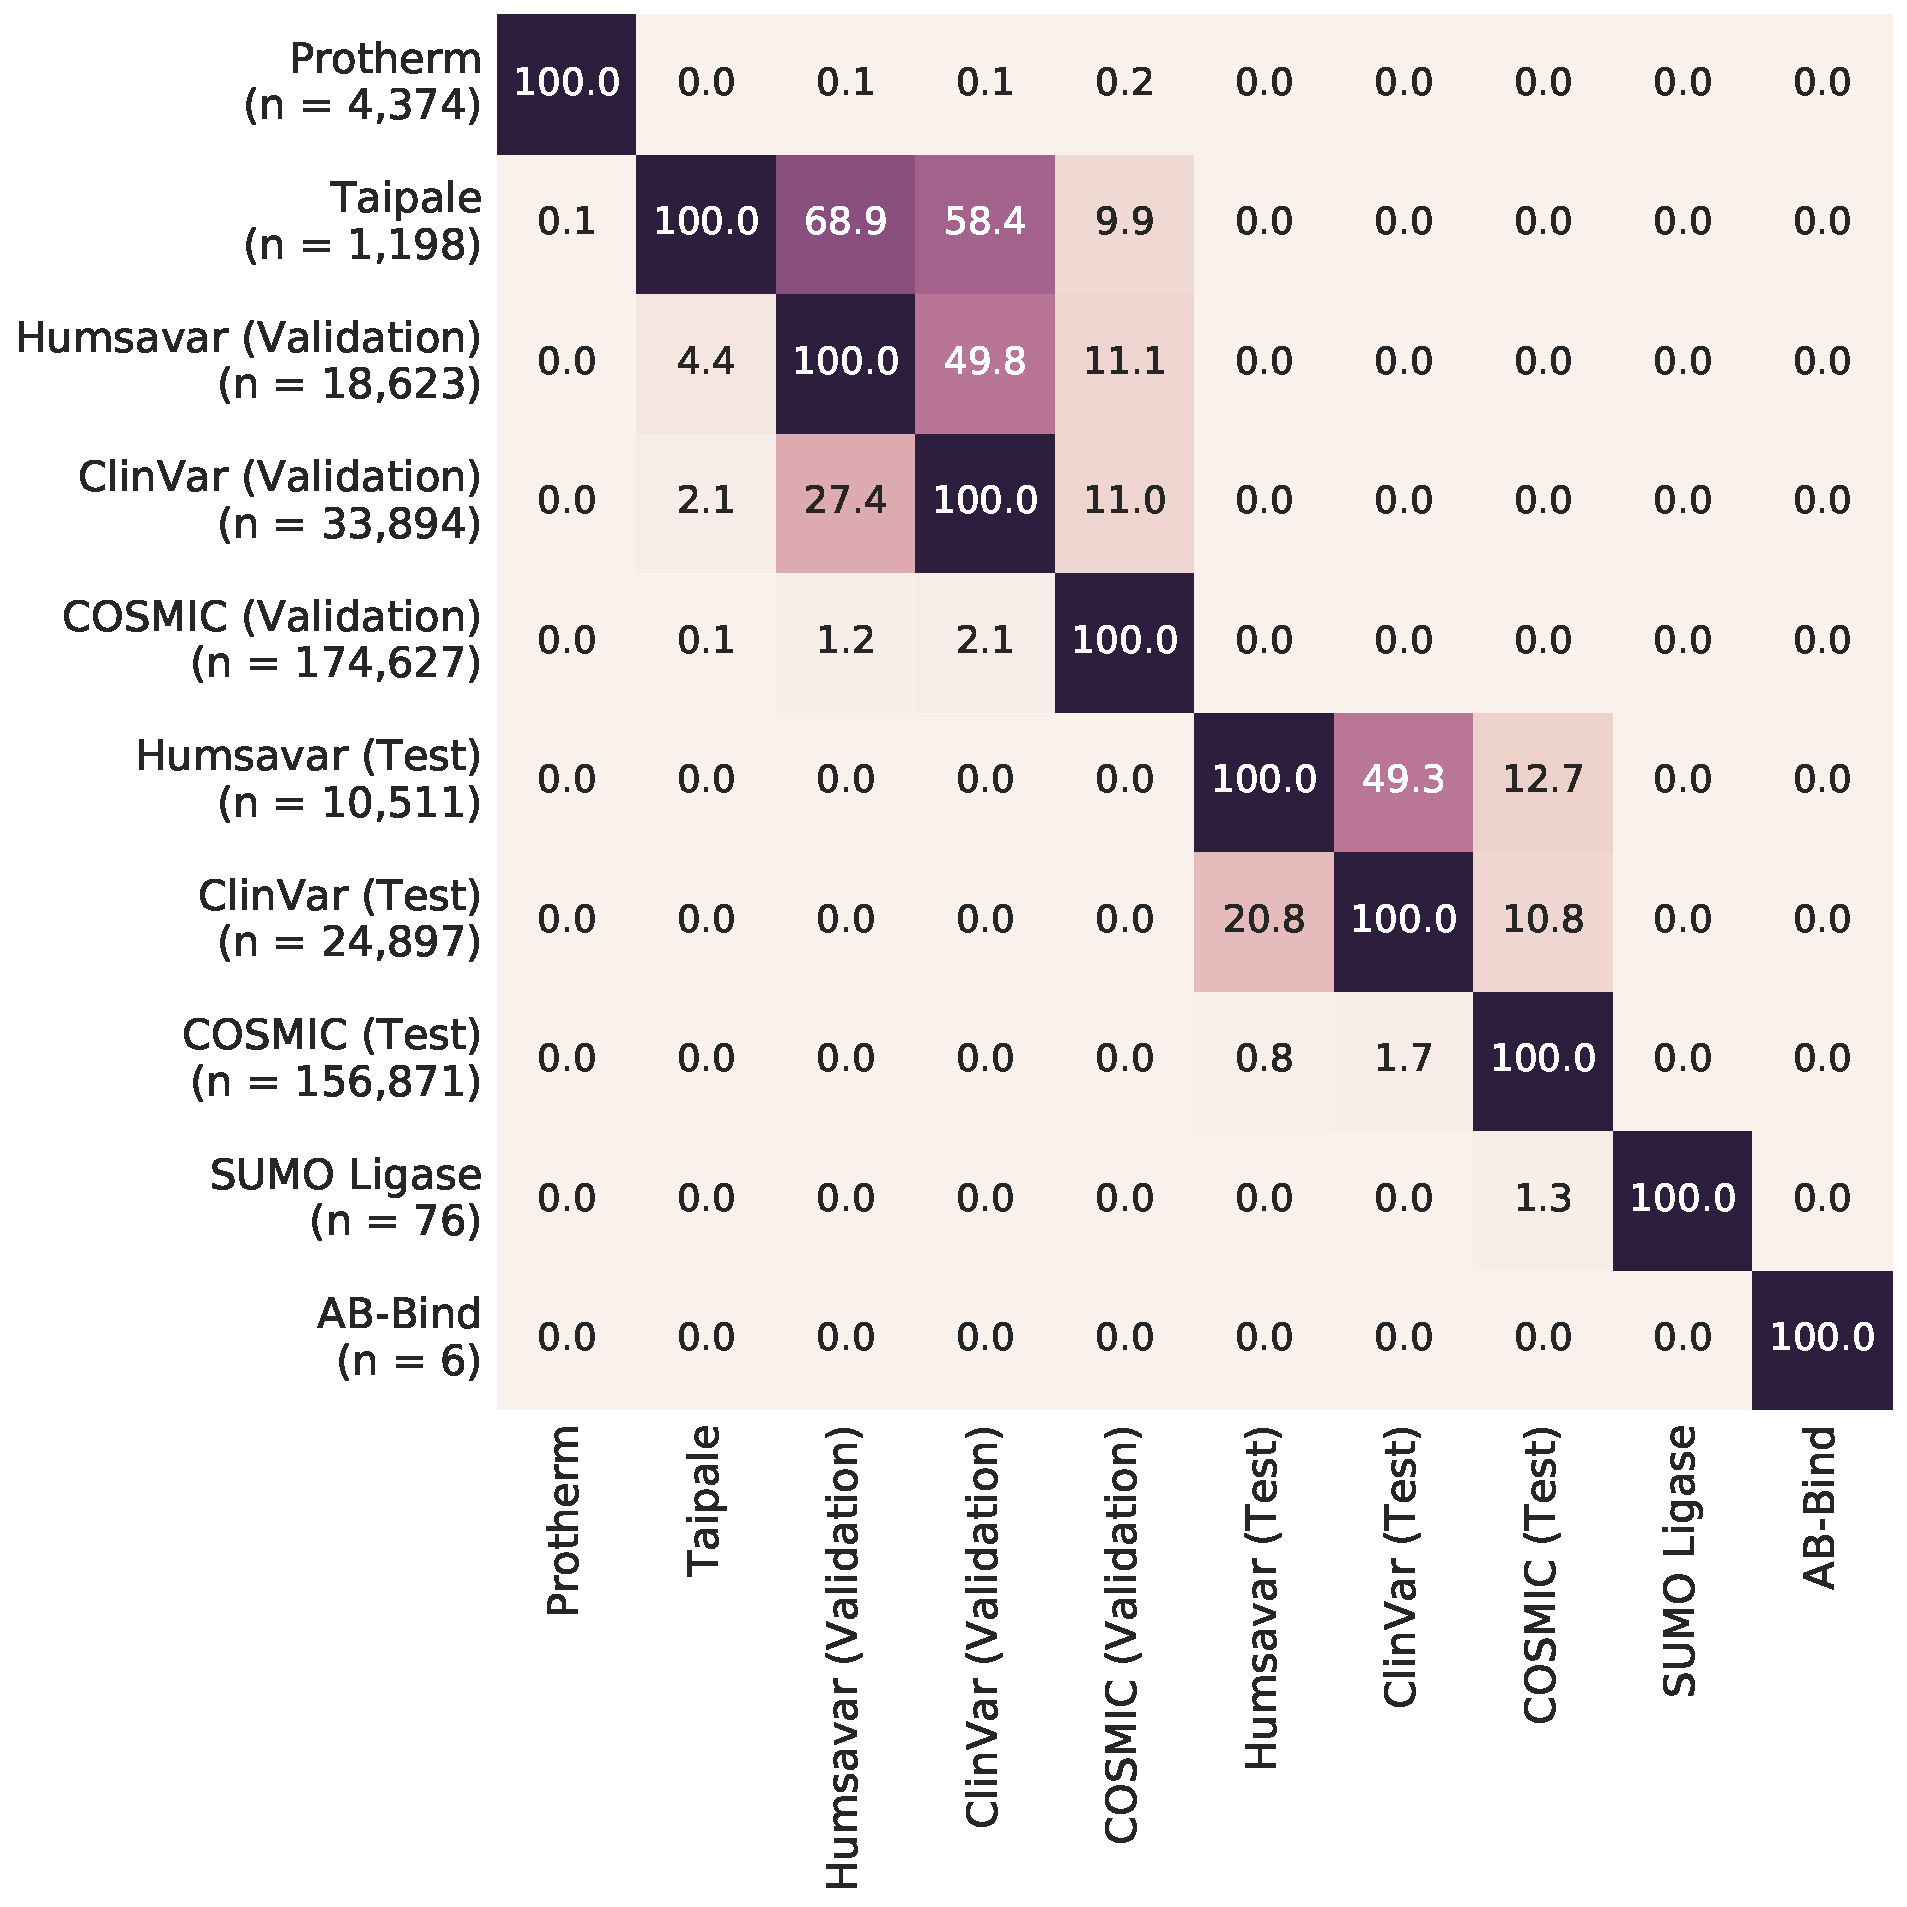
\includegraphics[width=0.8\textwidth]{static/elaspic_training_set/data_statistics/training_set_overlap_data_df_tt_core.pdf}
	\caption[Overlap in core mutation datasets.]{
		Overlap in core mutations between all the datasets used in this study.
		The shade and value inside each square denotes the percentage of mutations in the dataset named on the y-axis that are also found in the database named on the x-axis.
		Core mutations are defined as mutations that do not occur within 6 \AA of a neighbouring chain in the provided PDB or protein-protein homology model.
		A description of each dataset can be found in Table \ref{tab:datasets}.
	}
	\label{fig:training_set_overlap_core}
\end{figure}

\clearpage

\begin{figure}[tb]
	\centering
	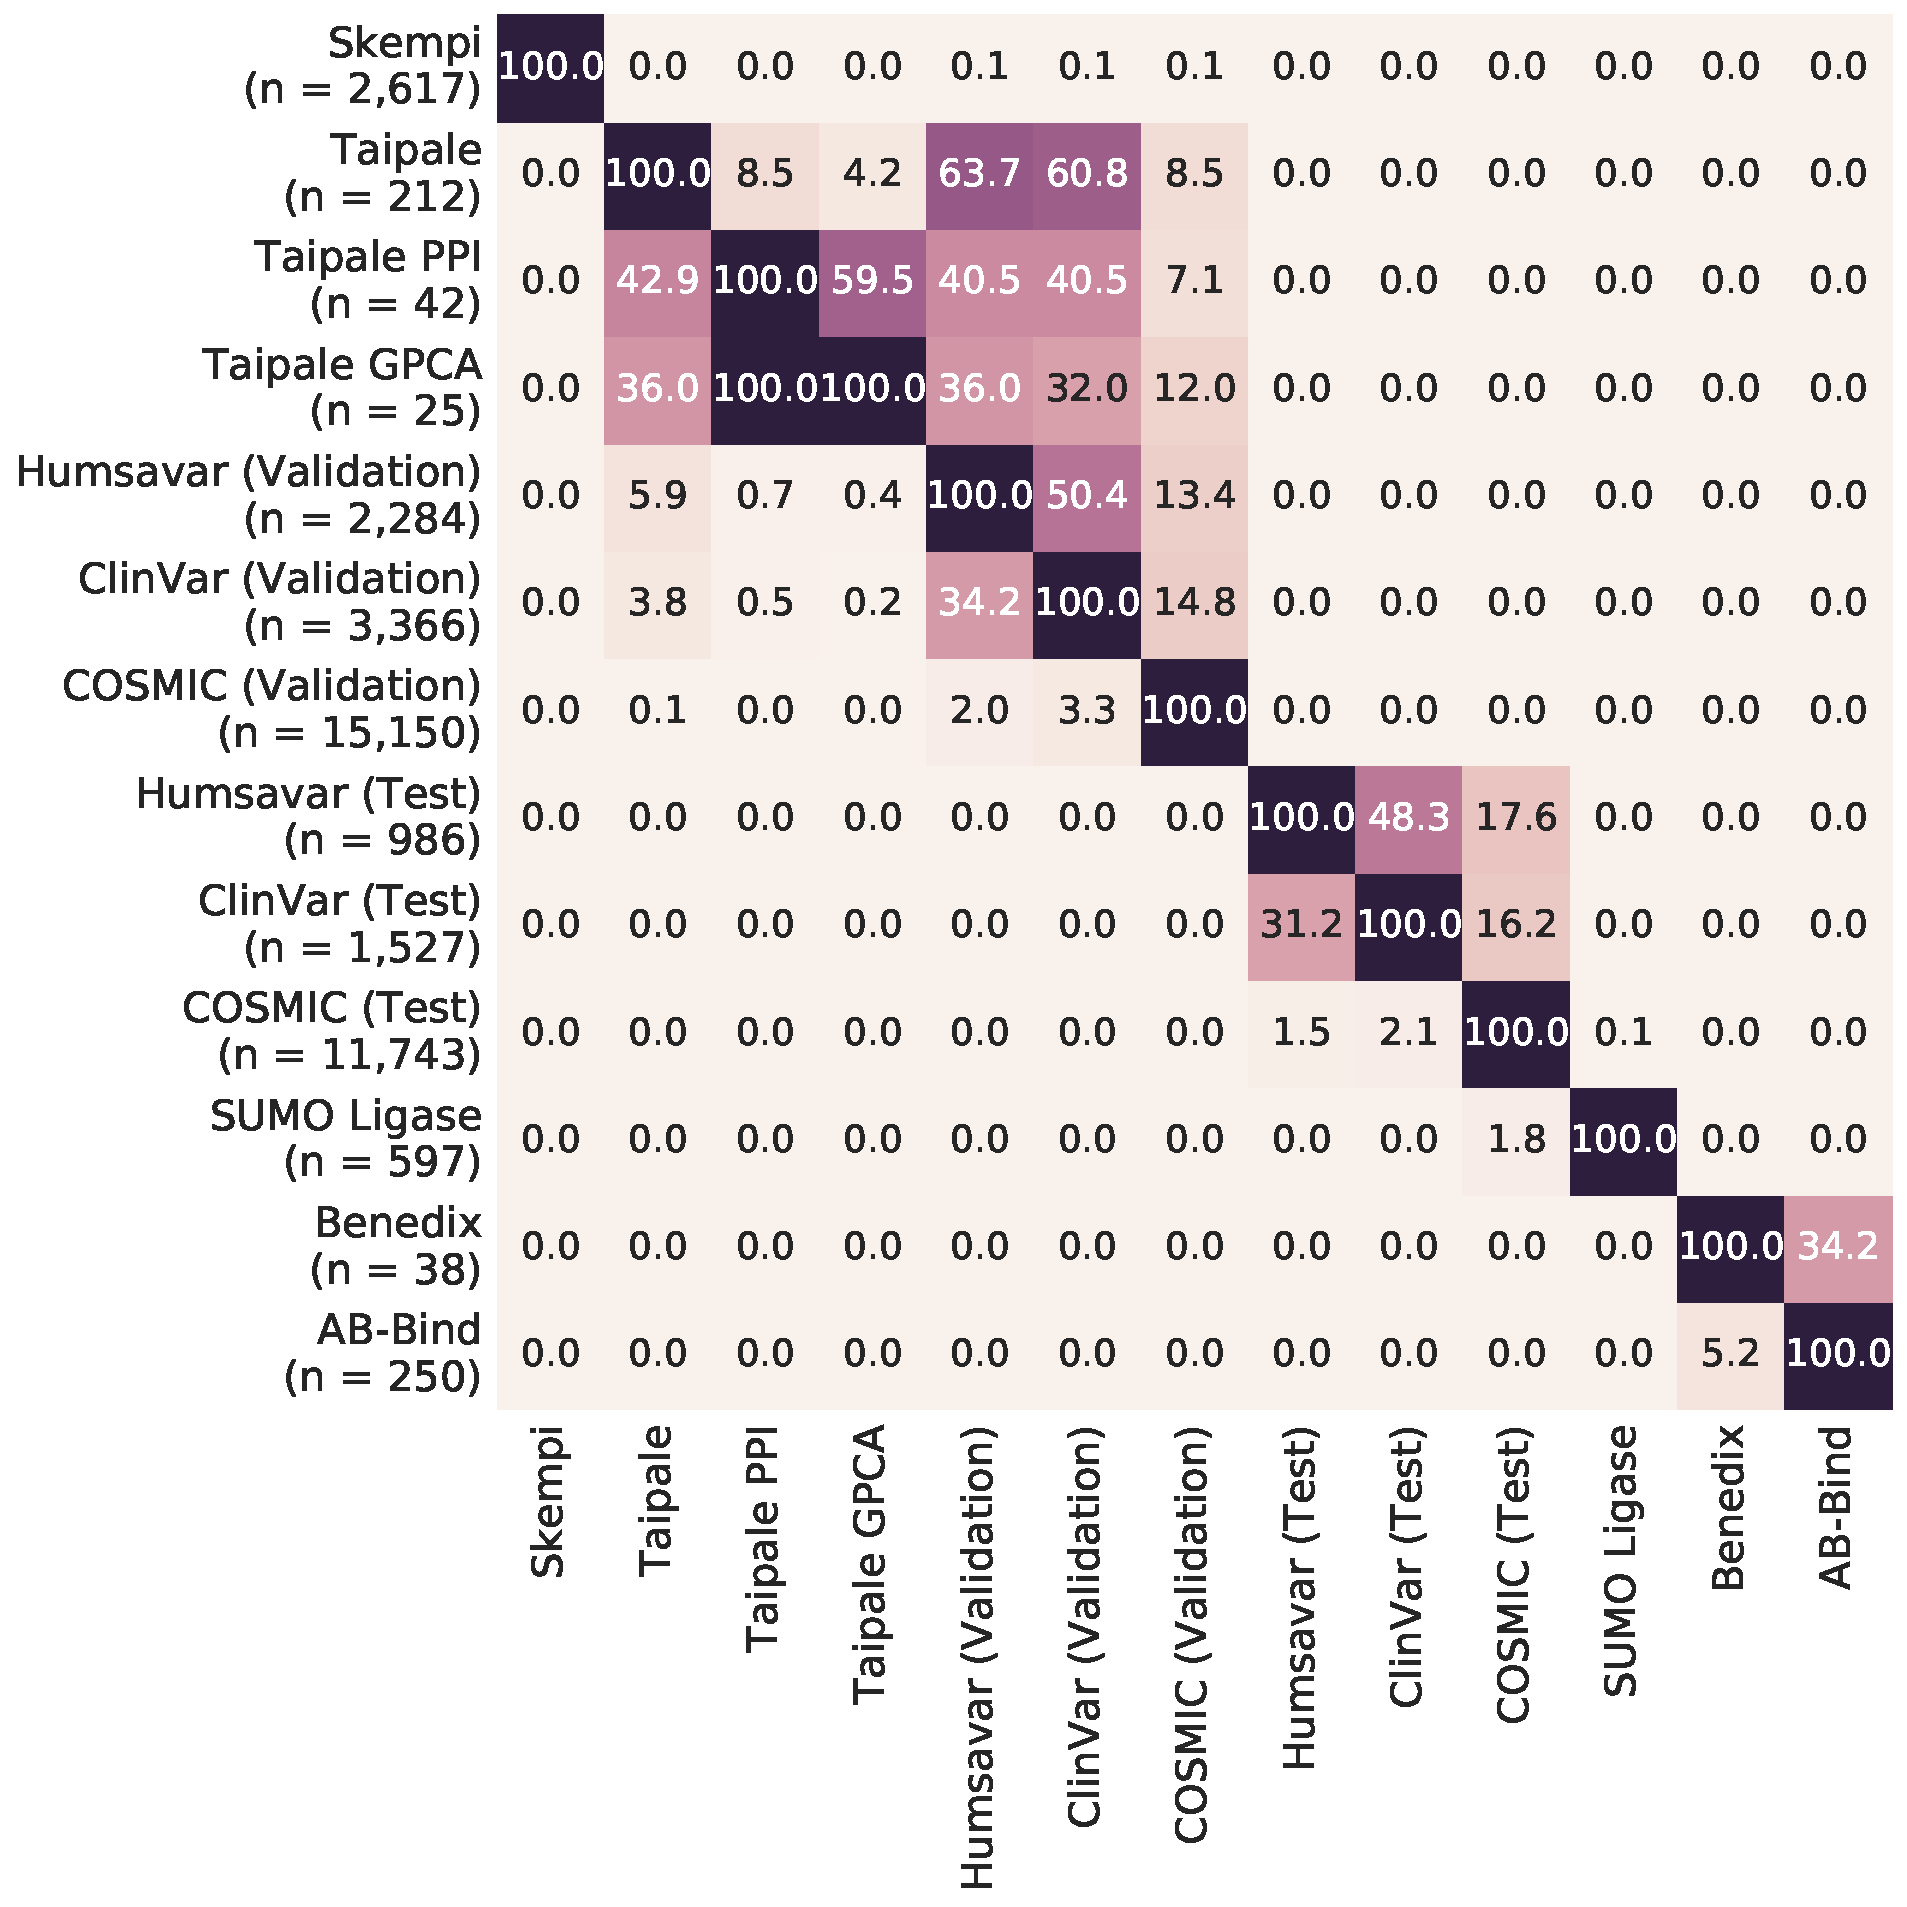
\includegraphics[width=0.9\textwidth]{static/elaspic_training_set/data_statistics/training_set_overlap_data_df_tt_interface.pdf}
	\caption[Overlap in interface mutation datasets.]{
		Overlap in interface mutations between all the datasets used in this study.
		The shade and value inside each square denotes the percentage of mutations in the dataset named on the y-axis that are also found in the database named on the x-axis.
		Interface mutations are defined as mutations that occur within 6 \AA of a neighbouring chain in the provided PDB or protein-protein homology model.
		A description of each dataset can be found in Table \ref{tab:datasets}.
	}
	\label{fig:training_set_overlap_interface}
\end{figure}



\clearpage
\section{Hyperparameter optimisation} \label{sec:gridsearch}

ELASPIC uses the gradient boosting regressor (GBR) algorithm, implemented in scikit-learn \cite{scikit-learn}, to  combine over 70 different sequential and structural features into a score that corresponds to the Gibbs free energy change of protein folding or protein-protein interaction. The GBR algorithm was selected because it achieved higher performance than linear regression, support vector machine and random forest algorithms, in 20-fold cross-validation over the training set \cite{berliner_combining_2014}.

Since the ELASPIC pipeline received many bugfixes since the original publication, and was restructured to work as a backend to a webserver, we retrained GBR predictors using features generated by the updated pipeline. In order to select the best set of GBR hyperparameters, we performed exhaustive ``grid-search'', where we measured the performance of the GBR algorithm for 3,600 different combinations of hyperparameters (Table \ref{tab:gridsearch_parameters}). For each set of parameters, we computed the Spearman correlation between predicted and experimental $\Delta \Delta G$ values for mutations in the training set, using 4-fold cross-validation. We also computed the Spearman correlation between predicted $\Delta \Delta G$ values and the measured values for our ``Validation'' datasets (datasets in Table \ref{tab:datasets} annotated as ``Validation''). In the case of the ``Taipale'' dataset, the experimental value was the difference in the average LUMIER score between the wildtype and mutant proteins and the corresponding chaperones. In the case of the ``Taipale PPI'' dataset, the experimental value was $1$ if the mutation led to the loss of the interaction and $0$ if it led to the gain of interaction or if it had no effect. In the case of the ``Taipale GPCA'' dataset, the experimental value was the difference in \textit{Gaussia princeps} luminosity between wild-type and mutant proteins. In the case of ``Humsavar'', ``ClinVar'' and ``COSMIC'' datasets, the experimental value was $1$ if the mutation was classified as deleterious and $0$ if it was classified as benign. While mutation deleteriousness and $\Delta \Delta G$ are different metrics, it is expected that deleterious mutations, on average, should have a higher impact on protein structure that benign mutations. Therefore, accurate $\Delta \Delta G$ predictions should have a higher correlation with the deleteriousness score, defined as $1$ for deleterious mutations and $0$ for benign mutations.

We used the combined scores $CS_{core}$ (Equations \ref{eq:combined_score_core}) and $CS_{interface}$ (Equation \ref{eq:combined_score_interface}) to select the best set of hyperparameters for the core and interface predictors. The contribution of each dataset to the combined score was selected in an ``ad-hoc'' manner, assigning more weight to large datasets than to small datasets, and making sure that the performance on energy-based datasets, including training and Taipale datasets, had a bigger overall impact on the combined score than performance on a deleteriousness-based datasets, such as Humsavar, ClinVar and COSMIC. We used combined scores instead of cross-validation alone because we wanted to select predictors that not only perform well on the training set, but also generalize to external datasets. Since our training sets are limited and biased in the number and type of proteins and protein-protein interactions that they contain, the performance of the predictor in cross-validation may not be an accurate indicator of its performance in general. Since our validation datasets contain many more distinct proteins, protein-protein interactions and mutations than our training sets, they offer a helpful indication of how well predictors generalize to other proteins in the human genome.

\begin{equation} \label{eq:combined_score_core}
    CS_{core} = \frac{3 \cdot Cross\_validation + Humsavar + ClinVar + COSMIC + Taipale}{7}
\end{equation}

\begin{equation} \label{eq:combined_score_interface}
    CS_{interface} = \frac{3 \cdot Cross\_validation + Humsavar + ClinVar + COSMIC + \frac{Taipale\_{PPI}}{4} + \frac{Taipale\_{GPCA}}{4}}{6.5}
\end{equation}

We plot the performance of core and interface predictors trained using different sets of hyperparameters and sorted according to the combined score in Figures \ref{fig:gridsearch_core} and \ref{fig:gridsearch_interface}. Cross-validation performance of the predictor is highly correlated with its performance on the validation datasets. However, selecting hyperparameters solely based on cross-validation performance would result in a predictor that substantially underperforms on the validation datasets.

\clearpage
% !TEX root = msc_thesis.tex

\begin{figure}[tb]
	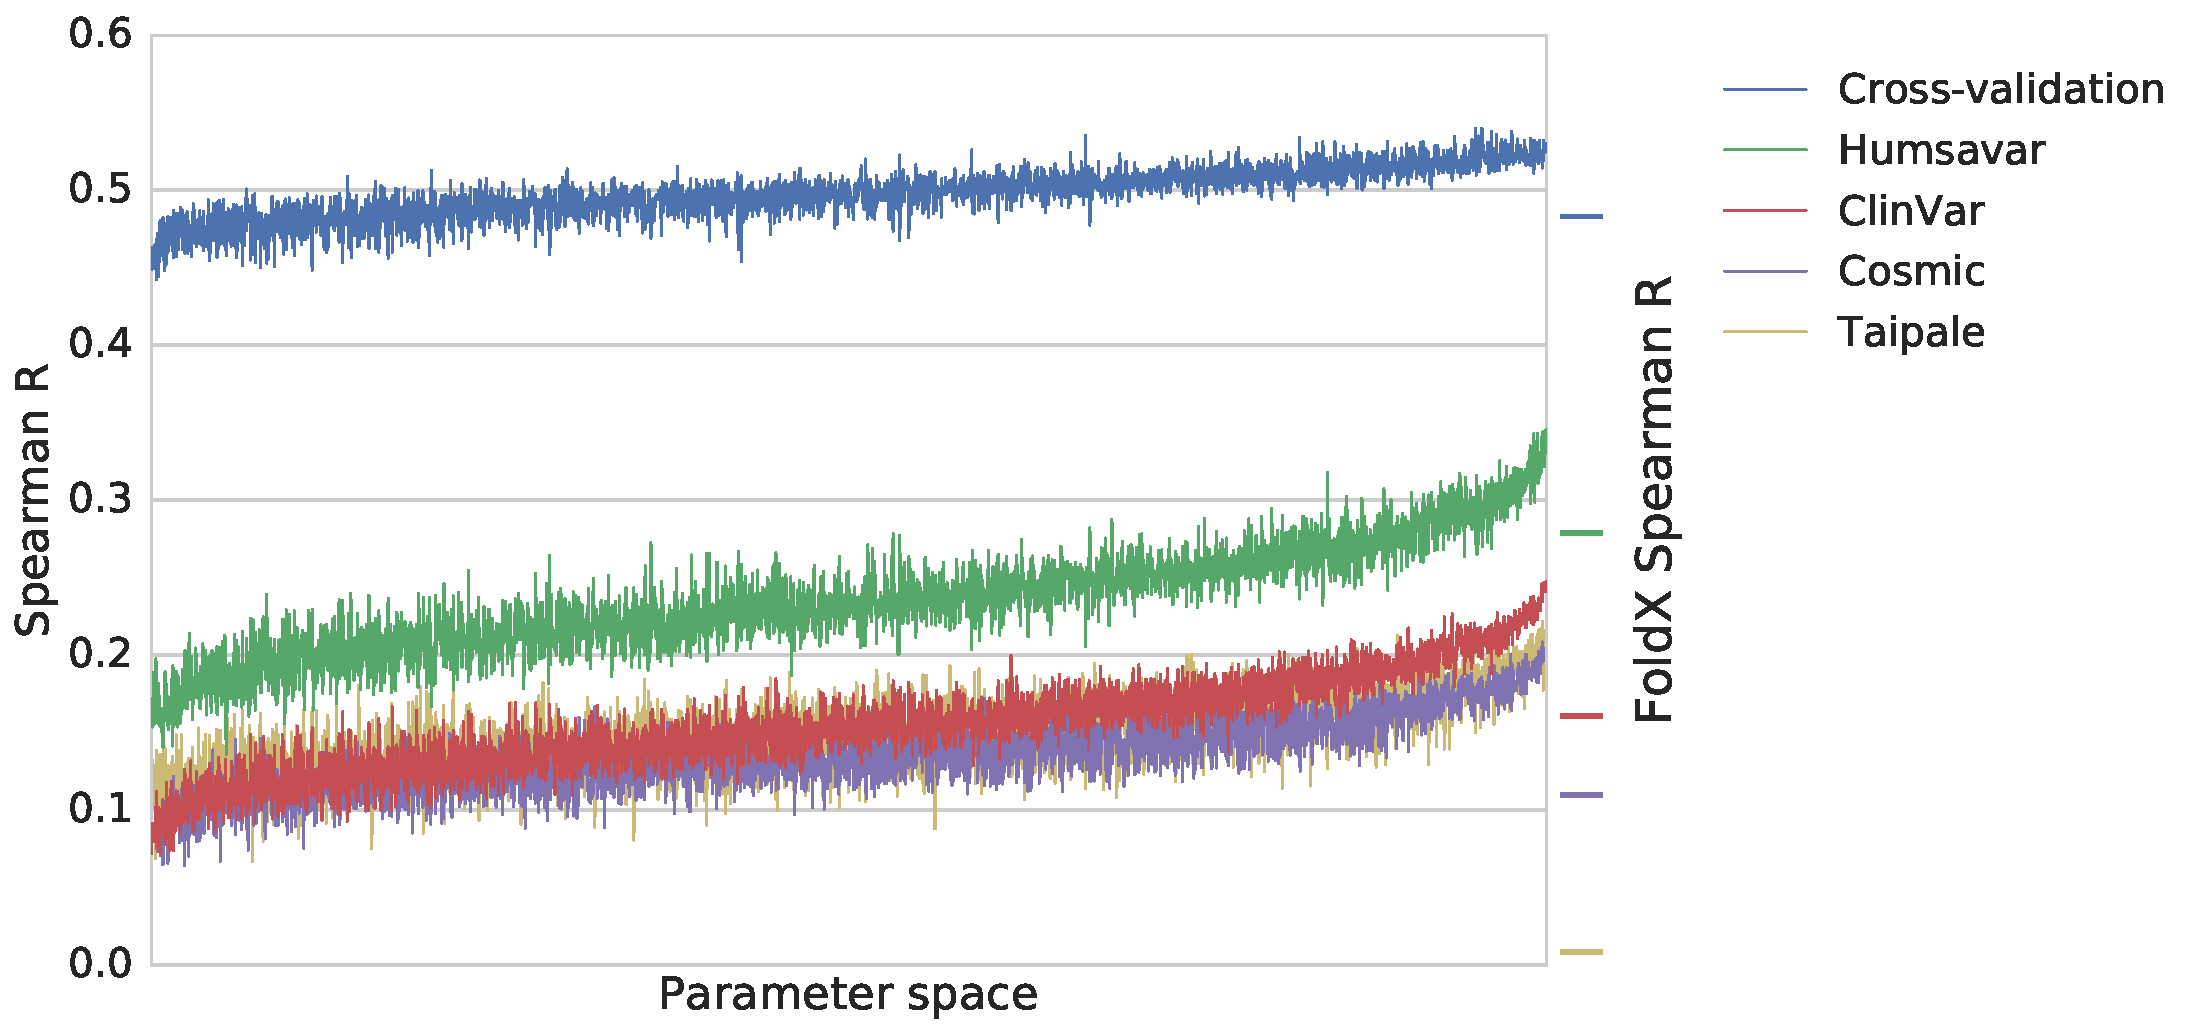
\includegraphics[width=0.9\linewidth]{static/elaspic_training_set/machine_learning/gridsearch_core.pdf}
	\caption[Core predictor hyperparameter optimization.]{
        Core predictor hyperparameter optimization.
        The combined score (black line) was calculated using Equation \ref{eq:combined_score_core}.
    }
	\label{fig:gridsearch_core}
\end{figure}

\begin{figure}[tb]
	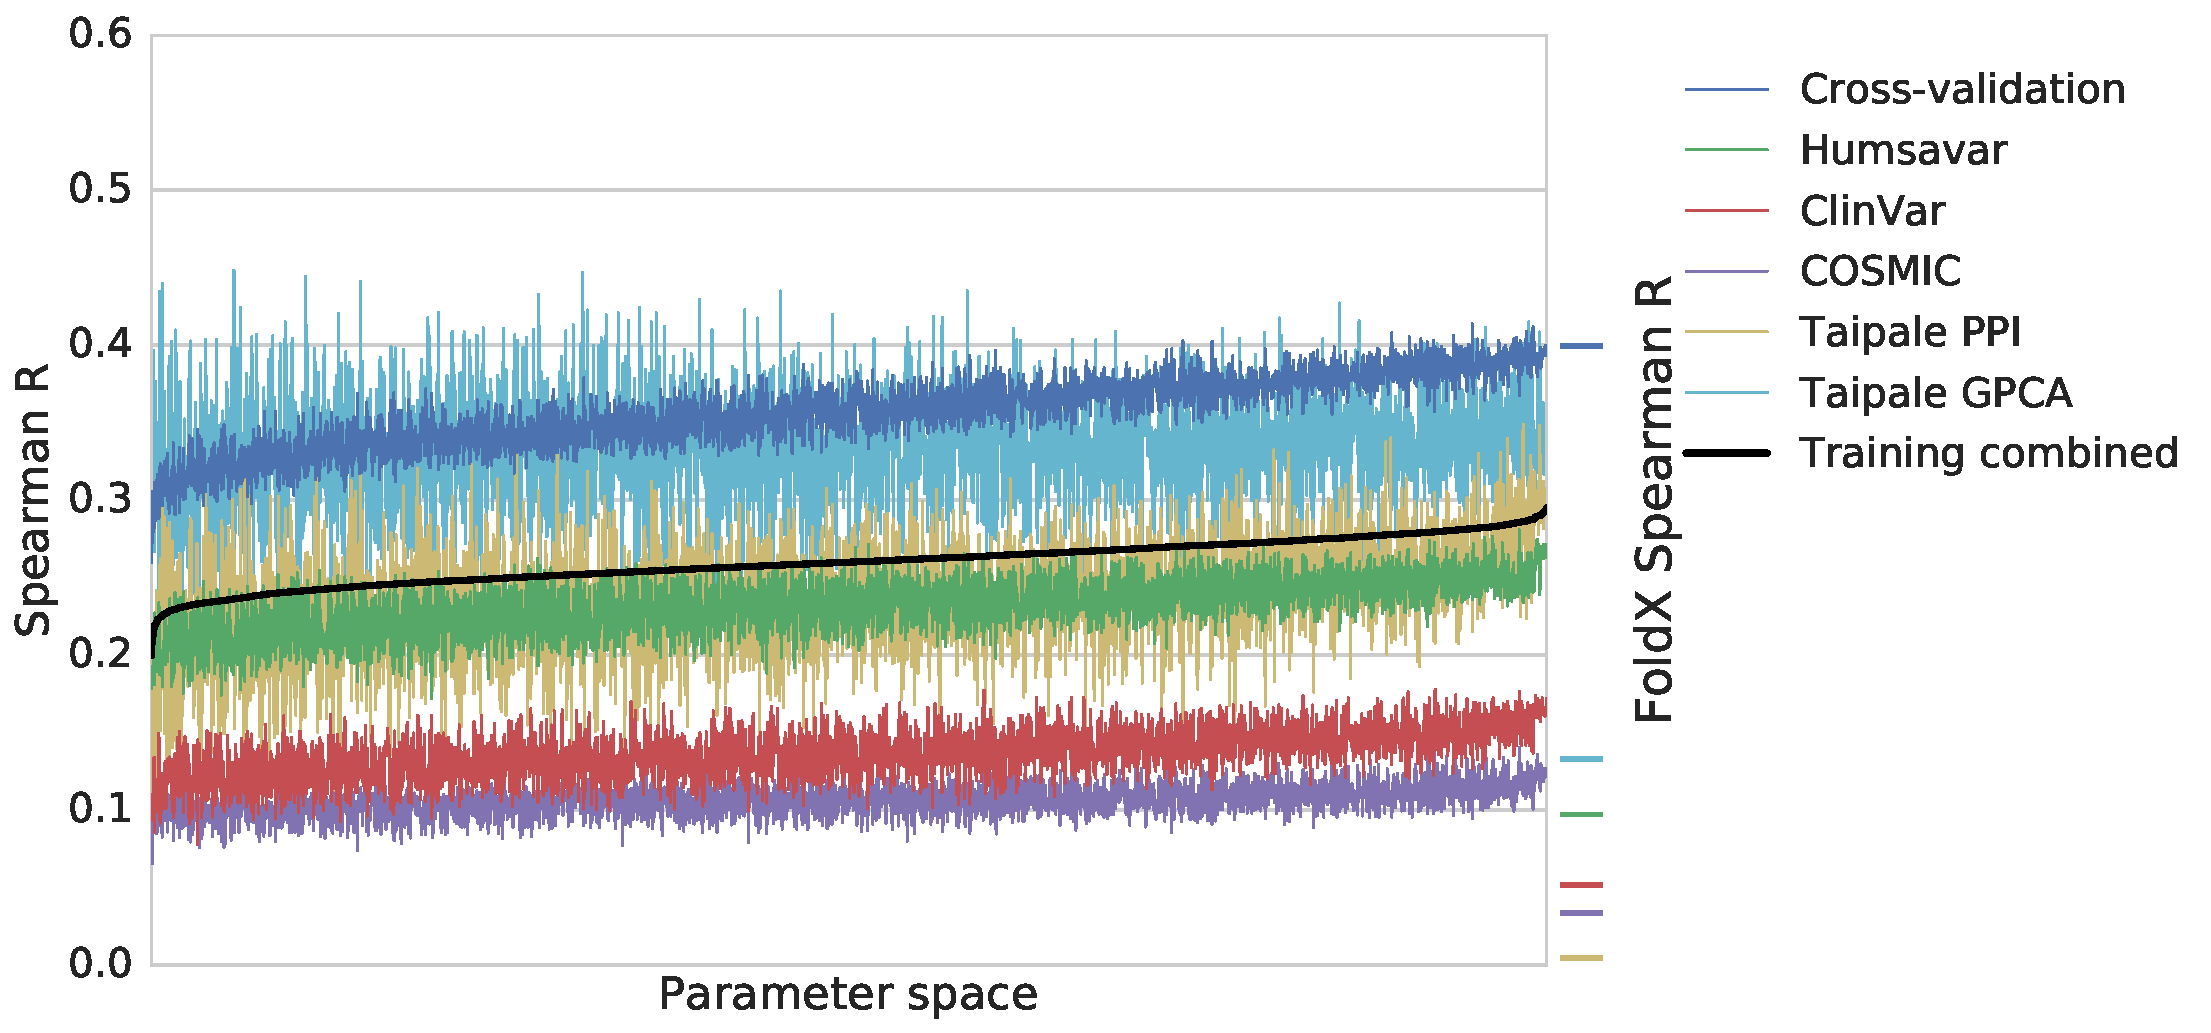
\includegraphics[width=0.9\linewidth]{static/elaspic_training_set/machine_learning/gridsearch_interface.pdf}
    \caption[Interface predictor hyperparameter optimization.]{
        Interface predictor hyperparameter optimization.
        The combined score (black line) was calculated using Equation \ref{eq:combined_score_interface}.
    }
	\label{fig:gridsearch_interface}
\end{figure}

\clearpage

\begin{table}[tb]
    \captionsetup{width=0.6\textwidth}
	\centering
	\caption[Hyperparameter search space.]{
        Hyperparameter search space for tuning the gradient boosting regressor algorithm used in the core and interface predictors. An all-by-all combination of these hyperparameters was explored in order to find those that produce the best-performing predictors.
    }
	\label{tab:gridsearch_parameters}
	\begin{tabular}{ l | l }
		\toprule
		Parameter name     & Parameter value                \\
		\midrule
		alpha              & 0.99, 0.95, 0.9, 0.8, 0.7, 0.5 \\
		learning\_rate     & 0.1, 0.05, 0.02, 0.01          \\
		loss               & huber                          \\
		max\_depth         & 10, 8, 6, 4                    \\
		max\_features      & 1.0, 0.8, 0.5, 0.3, 0.1,       \\
		min\_samples\_leaf & 29, 21, 17, 13, 9, 5, 3        \\
		n\_estimators      & 2000                           \\
		\bottomrule
	\end{tabular}
\end{table}

\begin{table}[tb]
	\centering
	\caption[Hyperparameters selected for the core predictor.]{
            Hyperparameters selected for the core predictor.
        }
    \label{tab:core_hyperparameters}
	\begin{tabular}{ l | l }
		\toprule
		Parameter name     & Parameter value \\
		\midrule
		alpha              & 0.5             \\
		learning\_rate     & 0.01            \\
		loss               & huber           \\
		max\_depth         & 4               \\
		max\_features      & 0.246           \\
		min\_samples\_leaf & 17              \\
		n\_estimators      & 2000            \\
		\bottomrule
	\end{tabular}
\end{table}

\begin{table}[tb]
	\centering
	\caption[Hyperparameters selected for the interface predictor.]{
            Hyperparameters selected for the interface predictor.
        }
	\label{tab:interface_hyperparameters}
	\begin{tabular}{ l | l }
		\toprule
		Parameter name     & Parameter value \\
		\midrule
		alpha              & 0.9             \\
		learning\_rate     & 0.01            \\
		loss               & huber           \\
		max\_depth         & 4               \\
		max\_features      & 0.3             \\
		min\_samples\_leaf & 13              \\
		n\_estimators      & 2000            \\
		\bottomrule
	\end{tabular}
\end{table}



\clearpage
\section{Feature elimination} \label{sec:feature_elimination}

After selecting the best set of hyperparameters for core and interface predictors, we performed feature elimination to evaluate the contribution of each feature to the overall accuracy of the predictor, and to select the sets of features that result in the most accurate predictions.

Feature elimination was performed using a recursive strategy, which involved:

\vspace{-\topsep}
\begin{itemize}
	\itemsep0em
	\item Leaving out each feature from the training set, one at a time.
	\item Training the predictor using all but the left out feature.
	\item Calculating the combined score ($CS_{core}$ or $CS_{interface}$) evaluating the performance of the predictor.
	\item Discarding the feature that, when left out, produced the predictor with the highest combined score.
	\item Repeating the process until only one feature remains.
\end{itemize}

Performances of the core and interface predictors at every step of feature elimination are shown in Figures \ref{fig:feature_elimination_core} and \ref{fig:feature_elimination_interface}. The sets of features that produced the best-performing predictors are described in Tables \ref{tab:core_features} and \ref{tab:interface_features}.

Most features play a surprisingly small role in the performance of the ELASPIC predictor. In fact, we can achieve near-optimal performance with both core and interface predictors by using only 6 features (displayed in bold in Tables \ref{tab:core_features} and \ref{tab:interface_features}). This suggests either that most features are not informative in predicting the energetic effect of mutations, or that the training set is too noisy for the contribution of those features to make a significant impact on the accuracy of the predictor.

\clearpage
% !TEX root = msc_thesis.tex

\begin{figure}[tb]
	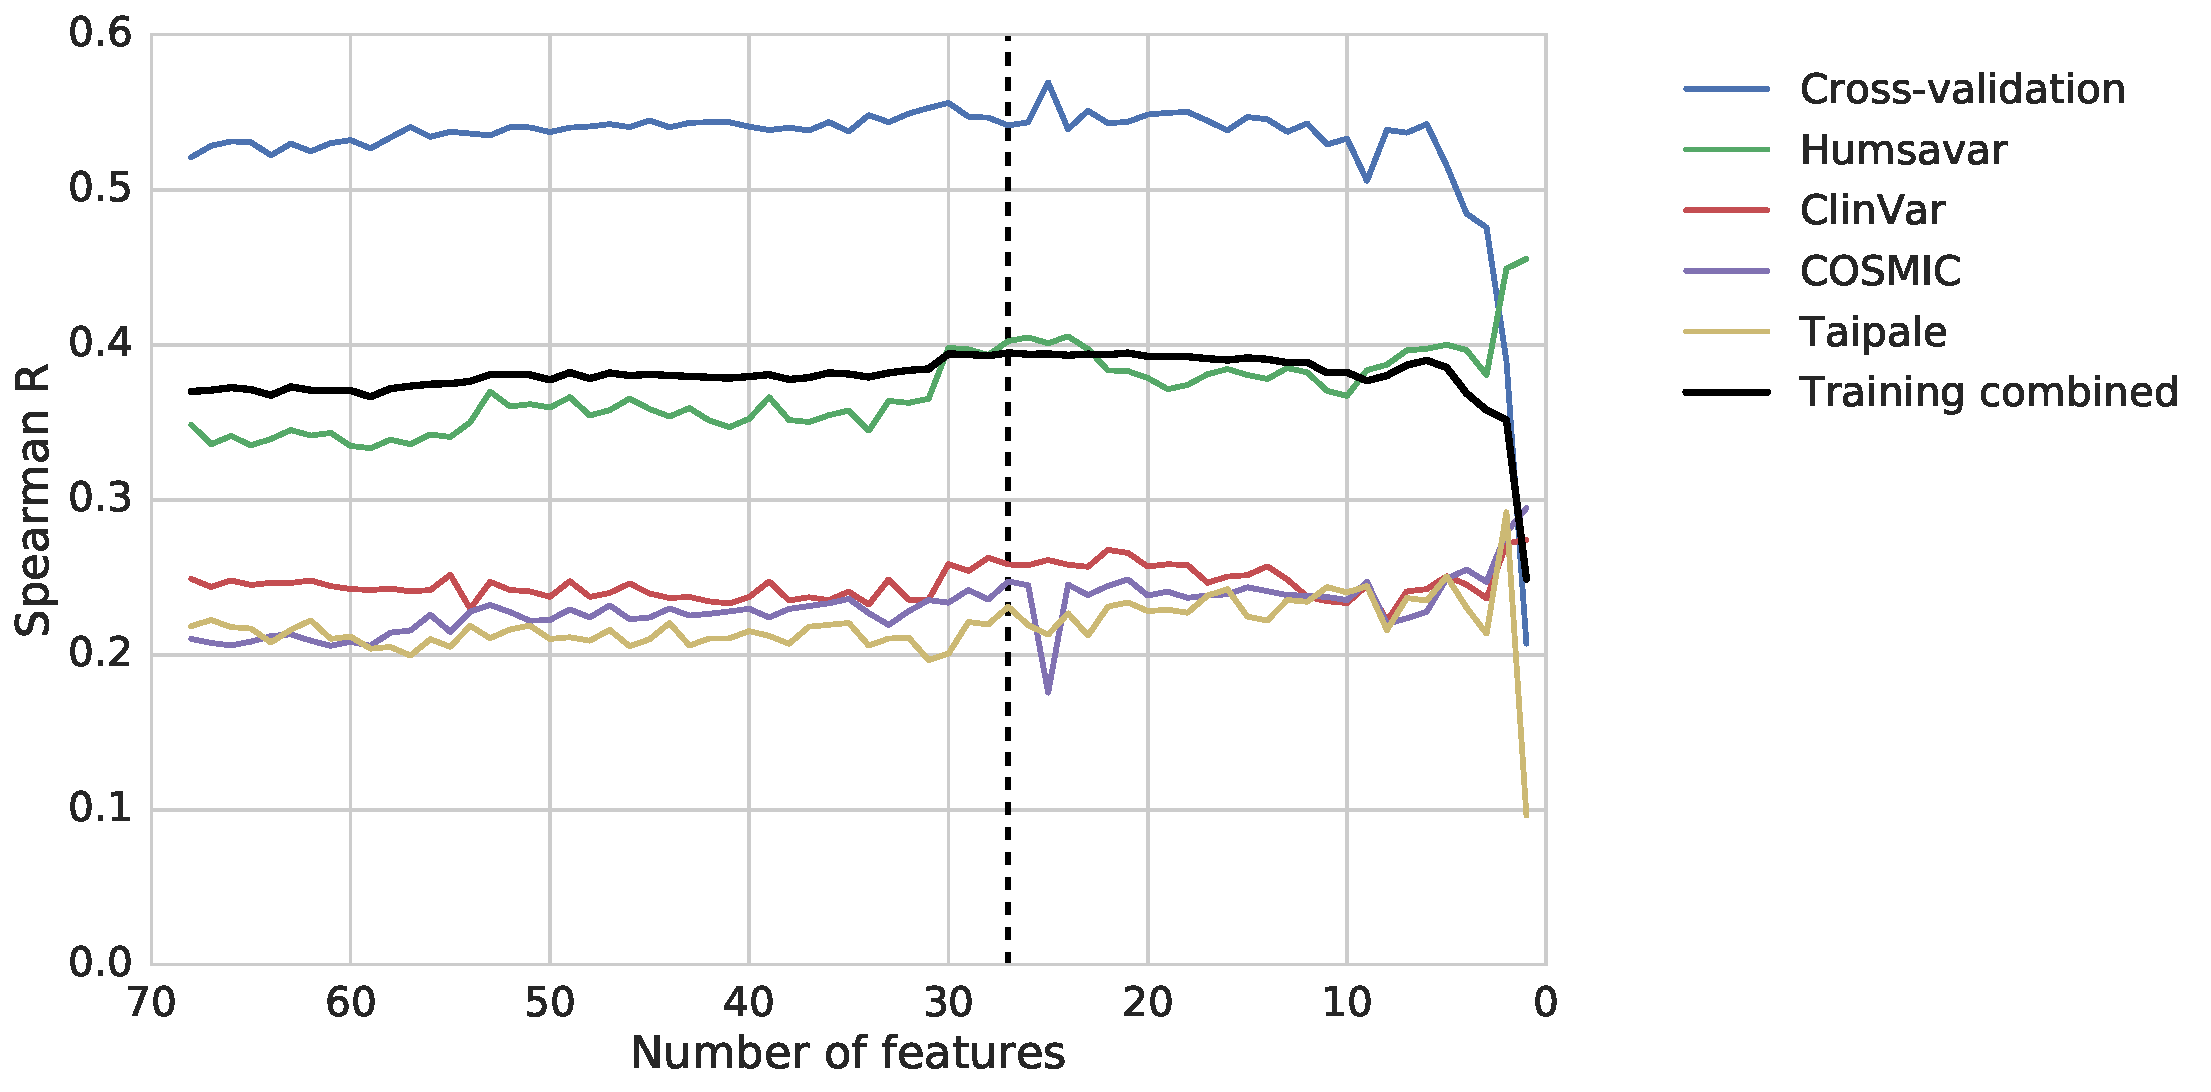
\includegraphics[width=0.9\linewidth]{static/elaspic_training_set/machine_learning/feature_elimination_core.pdf}
	\caption[Core predictor feature elimination.]{
		Performance of the core predictor at each step of feature elimination.
		The combined score (black line) was calculated using Equation \ref{eq:combined_score_core}.
		The set of features producing the predictor with the highest combined score are indicated by the vertical dashed line and are listed in Table \ref{tab:core_features}.
	}
	\label{fig:feature_elimination_core}
\end{figure}

\begin{figure}[tb]
	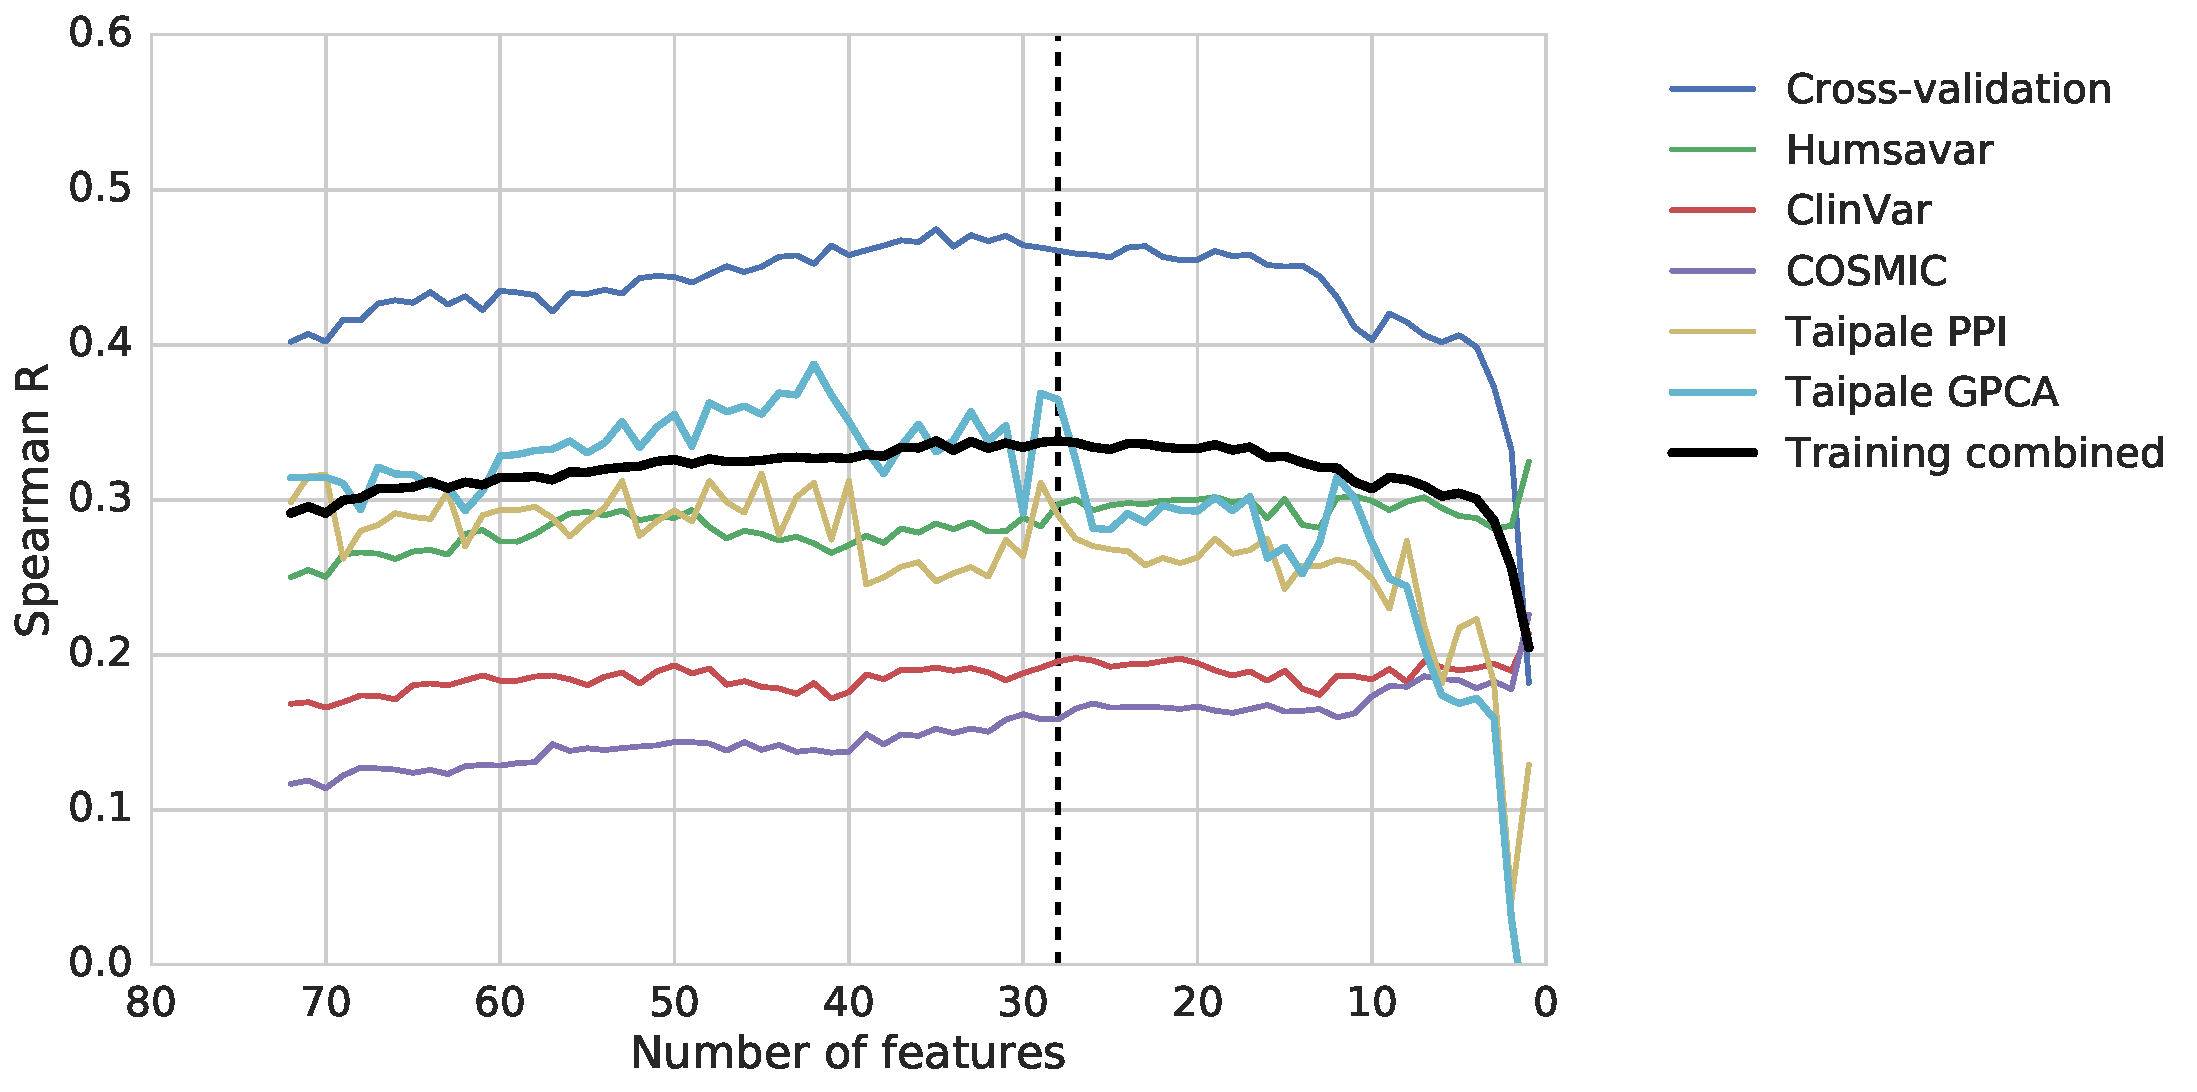
\includegraphics[width=0.9\linewidth]{static/elaspic_training_set/machine_learning/feature_elimination_interface.pdf}
	\caption[Interface predictor feature elimination.]{
		Performance of the interface predictor at each step of feature elimination.
		The combined score (black line) was calculated using Equation \ref{eq:combined_score_interface}.
		The set of features producing the predictor with the highest combined score are indicated by the vertical dashed line and are listed in Table \ref{tab:interface_features}.
	}
	\label{fig:feature_elimination_interface}
\end{figure}

\clearpage

\begin{table}[tb]
	\centering
	\caption[Features selected for the core predictor.]{
		Core predictor features.
		Features that end in \textit{\_wt} were computed for the wild-type structure.
		Features that end in \textit{\_change} correspond to the difference between the values computed for the wild-type and mutant structures.
		Rows in bold mark the 6 most important features.
		FoldX feature descriptions were taken from \url{http://foldxsuite.crg.eu/command/Stability}.
	}
	\label{tab:core_features}
	\begin{tabular}{ l | l | p{7cm} }
		\toprule
		Feature name                              & Feature source   & Feature description                                                                                 \\
		\midrule
		alignment\_coverage                       & ELASPIC          & Structural template alignment coverage.                                                             \\
		alignment\_identity                       & ELASPIC          & Structural template sequence identity.                                                              \\
		alignment\_score                          & ELASPIC          & Structural template quality (Equation \ref{eq:core_alignment_score}).                               \\
		backbone\_hbond\_change                   & FoldX            & Backbone hydrogen bond energy.                                                                      \\
		backbone\_hbond\_wt                       & FoldX            & This the contribution of backbone hydrogen bonds.                                                   \\
		cis\_bond\_wt                             & FoldX            & Cis peptide bond energy.                                                                            \\
		disulfide\_wt                             & FoldX            & Contribution of disulfide bonds.                                                                    \\
		electrostatic\_kon\_change                & FoldX            & Electrostatic interaction between molecules in the pre-complex.                                     \\
		\textbf{electrostatics\_change}           & \textbf{FoldX}   & \textbf{Electrostatic interactions.}                                                                \\
		entropy\_mainchain\_change                & FoldX            & Entropy cost of fixing the main chain.                                                              \\
		helix\_dipole\_wt                         & FoldX            & Electrostatic contribution of the helix dipole.                                                     \\
		matrix\_score                             & ELASPIC          & BLOSUM62 matrix score.                                                                              \\
		pcv\_hbond\_change                        & ELASPIC          & Hydrogen-oxygen contacts involving atoms of the mutated residue and atoms of the interacting chain. \\
		pcv\_hbond\_self\_change                  & ELASPIC          & Hydrogen-oxygen contacts involving atoms of the mutated residue and atoms of the mutated chain.     \\
		pcv\_salt\_equal\_change                  & ELASPIC          & Charge repulsions between atoms of the mutated residue and atoms of the interacting chain.          \\
		pcv\_salt\_equal\_self\_wt                & ELASPIC          & Charge repulsions between atoms of the mutated residue and atoms of the mutated chain.              \\
		pcv\_salt\_equal\_wt                      & ELASPIC          & Charge repulsions between atoms of the mutated residue and atoms of the interacting chain.          \\
		pcv\_salt\_opposite\_change               & ELASPIC          & Charge attractions between atoms of the mutated residue and atoms of the interacting chain.         \\
		pcv\_vdw\_self\_change                    & ELASPIC          & Carbon carbon contacts between atoms of the mutated residue and atoms of the mutated chain.         \\
		\textbf{provean\_score}                   & \textbf{Provean} & \textbf{Sequence conservation score.}                                                               \\
		sloop\_entropy\_wt                        & FoldX            & Entropic cost according to the SLoop database of loop conformations.                                \\
		\textbf{solvation\_hydrophobic\_change}   & \textbf{FoldX}   & \textbf{Contribution of hydrophobic groups.}                                                        \\
		\textbf{solvation\_polar\_change}         & \textbf{FoldX}   & \textbf{Energetic penalty for burying polar groups.}                                                \\
		\textbf{solvent\_accessibility\_wt}       & \textbf{MSMS}    & \textbf{Solvent-accessible surface area of the mutated residue.}                                    \\
		torsional\_clash\_change                  & FoldX            & Intra-residue van der Waals torsional clashes.                                                      \\
		\textbf{van\_der\_waals\_clashes\_change} & \textbf{FoldX}   & \textbf{Energy penalization due to van der Waals clashes (interresidue).}                           \\
		water\_bridge\_wt                         & FoldX            & Contribution of water bridges.                                                                      \\
		\bottomrule
	\end{tabular}
\end{table}

\begin{table}[tb]
	\centering
	\caption[Features selected for the interface predictor.]{
		Interface predictor features.
		Features that end in \textit{\_wt} were computed for the wild-type structure.
		Features that end in \textit{\_change} correspond to the difference between the values computed for the wild-type and mutant structures.
		Rows in bold mark the 6 most important features.
		FoldX feature descriptions were taken from \url{http://foldxsuite.crg.eu/command/AnalyseComplex}.
	}
	\label{tab:interface_features}
	\begin{tabular}{ l | l | p{8cm} }
		\toprule
		Feature name                          & Feature source   & Feature description                                                                                        \\
		\midrule
		alignment\_score                      & ELASPIC          & Alignment quality (Equation \ref{eq:interface_alignment_score}).                                           \\
		backbone\_clash\_change               & FoldX            & Backbone-backbone van der Waals energy.                                                                    \\
		backbone\_clash\_wt                   & FoldX            & Backbone-backbone van der Waals energy.                                                                    \\
		backbone\_hbond\_change               & FoldX            & Backbone hydrogen bond energy.                                                                             \\
		cis\_bond\_wt                         & FoldX            & Cis peptide bond energy.                                                                                   \\
		electrostatic\_kon\_wt                & FoldX            & Electrostatic interaction between molecules in the pre-complex.                                            \\
		energy\_ionisation\_wt                & FoldX            & Ionization energy.                                                                                         \\
		entropy\_complex\_change              & FoldX            & Entropic cost of forming a complex.                                                                        \\
		\textbf{entropy\_sidechain\_change}   & \textbf{FoldX}   & \textbf{Entropic cost of fixing the side chain.}                                                           \\
		intraclashes\_energy\_2\_change       & FoldX            & van der Waals clashes of residues at the interface of the complex with their own molecule (type 2).        \\
		\textbf{partial\_covalent\_bonds\_wt} & \textbf{FoldX}   & \textbf{Interactions with bound metals.}                                                                   \\
		pcv\_hbond\_self\_change              & ELASPIC          & Hydrogen-oxygen contacts involving atoms of the mutated residue and atoms of the mutated chain.            \\
		pcv\_hbond\_wt                        & ELASPIC          & Hydrogen-oxygen contacts involving atoms of the mutated residue and atoms of the interacting chain.        \\
		pcv\_salt\_equal\_self\_change        & ELASPIC          & Charge repulsions involving atoms of the mutated residue and atoms of the mutated chain.                   \\
		pcv\_salt\_equal\_wt                  & ELASPIC          & Charge repulsions involving atoms of the mutated residue and atoms of the interacting chain.               \\
		pcv\_salt\_opposite\_change           & ELASPIC          & Charge attractions involving atoms of the mutated residue and atoms of the interacting chain.              \\
		pcv\_salt\_opposite\_self\_change     & ELASPIC          & Charge attractions involving atoms of the mutated residue and atoms of the mutated chain.                  \\
		pcv\_salt\_opposite\_self\_wt         & ELASPIC          & Charge attractions involving atoms of the mutated residue and atoms of the mutated chain.                  \\
		pcv\_vdw\_self\_change                & ELASPIC          & Carbon carbon contacts involving atoms of the mutated residue and atoms of the mutated chain.              \\
		\textbf{pcv\_vdw\_self\_wt}           & \textbf{ELASPIC} & \textbf{Carbon carbon contacts involving atoms of the mutated residue and atoms of the mutated chain.}     \\
		\textbf{pcv\_vdw\_wt}                 & \textbf{ELASPIC} & \textbf{Carbon carbon contacts involving atoms of the mutated residue and atoms of the interacting chain.} \\
		\textbf{provean\_score}               & \textbf{Provean} & \textbf{Sequence conservation score.}                                                                      \\
		sloop\_entropy\_change                & FoldX            & Entropic cost according to the SLoop database of loop conformations.                                       \\
		solvation\_hydrophobic\_change        & FoldX            & Contribution of hydrophobic groups.                                                                        \\
		\textbf{solvation\_polar\_change}     & \textbf{FoldX}   & \textbf{Energetic penalty for burying polar groups.}                                                       \\
		solvation\_polar\_wt                  & FoldX            & Energetic penalty for burying polar groups.                                                                \\
		torsional\_clash\_change              & FoldX            & Intra-residue van der Waals torsional clashes.                                                             \\
		water\_bridge\_change                 & FoldX            & Contribution of water bridges.                                                                             \\
		\bottomrule
	\end{tabular}
\end{table}



\clearpage
\section{Validation} \label{sec:validation}

The final ELASPIC core and interface predictors were trained using gradient boosting regressor hyperparameters listed in Tables \ref{tab:core_hyperparameters} and \ref{tab:core_features} and sets of features described in Tables \ref{tab:interface_hyperparameters} and \ref{tab:interface_features}. Performance of the resulting predictors on the training, validation and test datasets are presented in Figures \ref{fig:core_validation} and \ref{fig:interface_validation}, for core and interface predictors, respectively.

The ELASPIC core predictor outperforms FoldX and Provean on the Taipale dataset, which is the only validation dataset explicitly measuring the effect of mutations on protein stability rather than whether or not the mutation is associated with a disease (Figure \ref{fig:validation_performance_core}). It also outperforms FoldX and Provean on the core subsets of the SUMO and AB-Bind test datasets (Figure \ref{fig:test_performance_core}). The core subsets of those datasets only contain mutations located more than 6 {\AA} away from another chain in the PDB.

The ELASPIC interface predictor also outperforms FoldX and Provean on the Taipale GPCA dataset (Figure \ref{fig:validation_performance_interface}). It performs marginally worse than Provean on the Taipale PPI dataset, but this is likely because the Taipale PPI dataset is mostly made up of deleterious mutations, which are predicted well by Protherm. The ELASPIC interface outperforms Protherm and FoldX on the SUMO Ligase and AB-Bind test datasets (Figure \ref{fig:test_performance_interface}) both alone and in combination with the core predictor. The ELASPIC interface predictor shows slightly lower performance than FoldX on the very small Benedix dataset.

Both the core and interface predictors performs better than FoldX but worse than Provean on the validation and test subsets of the Humsavar, ClinVar and COSMIC (Figures \ref{fig:test_performance_core} and \ref{fig:test_performance_interface}). The low performance of the ELASPIC compared to Provean was expected, since the ELASPIC core predictor attempts to model the effect of mutations on protein stability, and does not account for other reasons that may lead to a mutation being deleterious. For example, mutations could affect the active site or the signal sequence of a protein, which may prove to be highly deleterious to the organism but have only a marginal effect on protein stability.




\clearpage
% !TEX root = msc_thesis.tex

\begin{figure}[tb]
	\centering
	\begin{subfigure}[b]{1.0\textwidth}
		\centering
		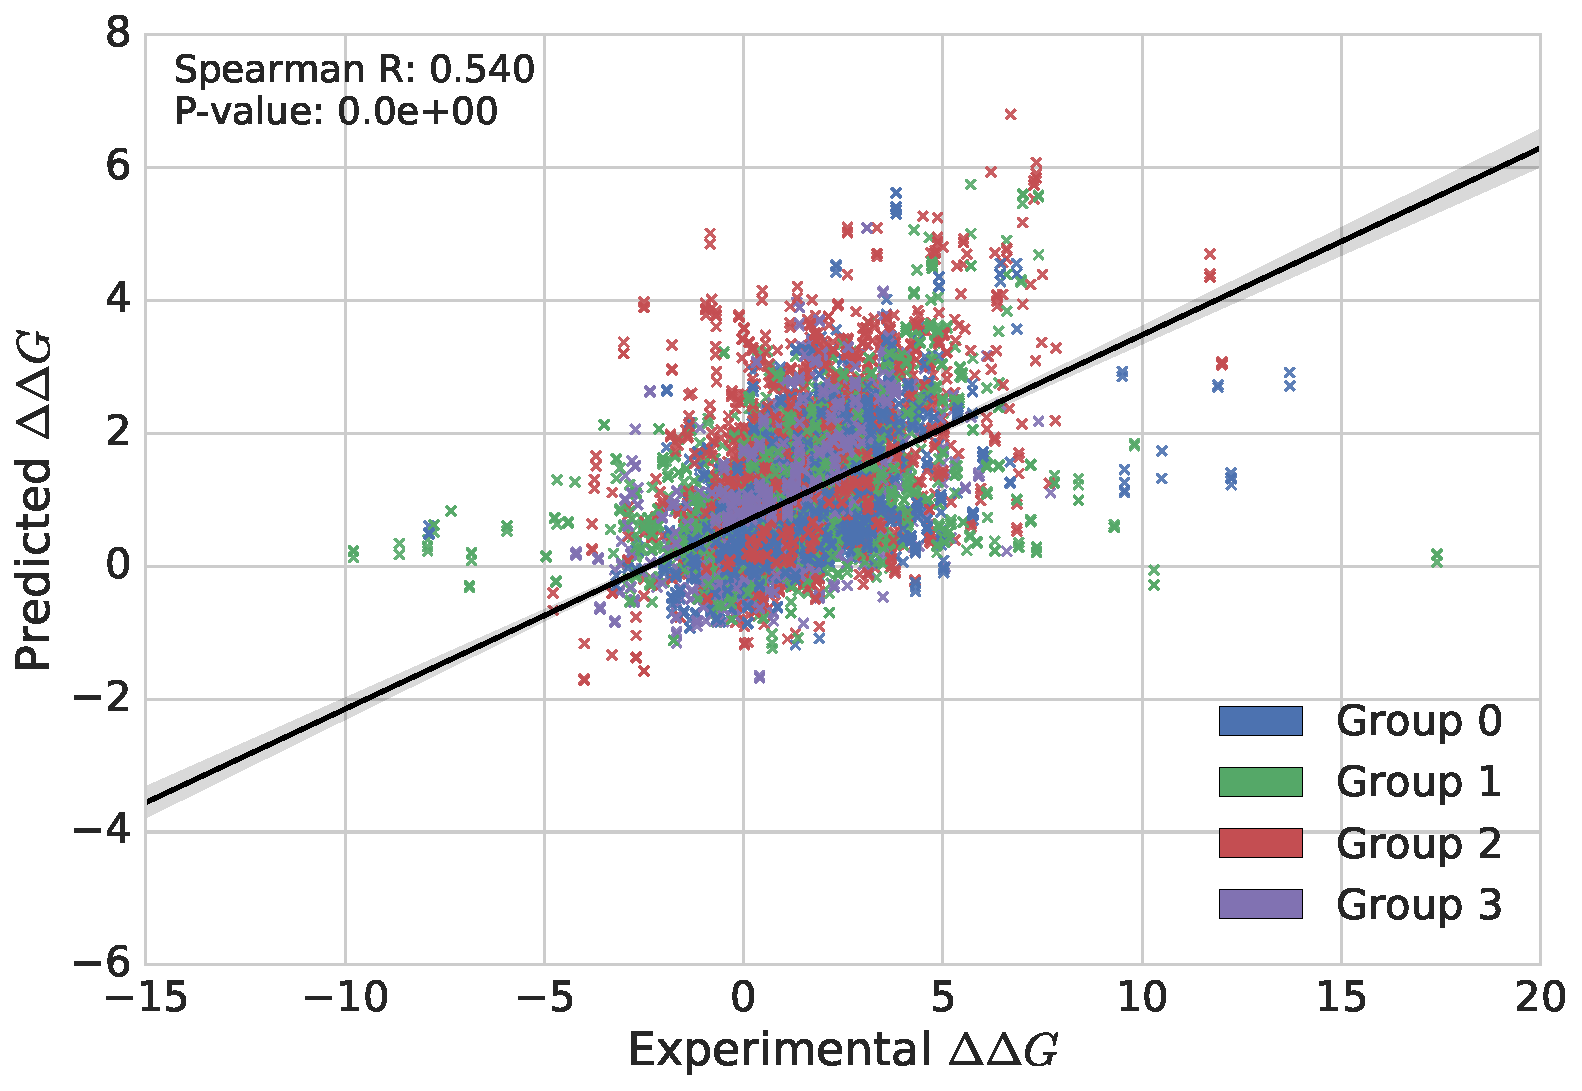
\includegraphics[width=0.6\linewidth]{static/elaspic_training_set/validation/crossvalidation_performance_core.pdf}
		\caption{
			Performance of the ELASPIC core predictor on the training dataset, evaluated using four-fold cross-validation.
			Colours indicate different cross-validation bins.
		}
		\label{fig:crossvalidation_performance_core}
		\vspace*{10mm}
	\end{subfigure}
	\begin{subfigure}[b]{1.0\textwidth}
		\centering
		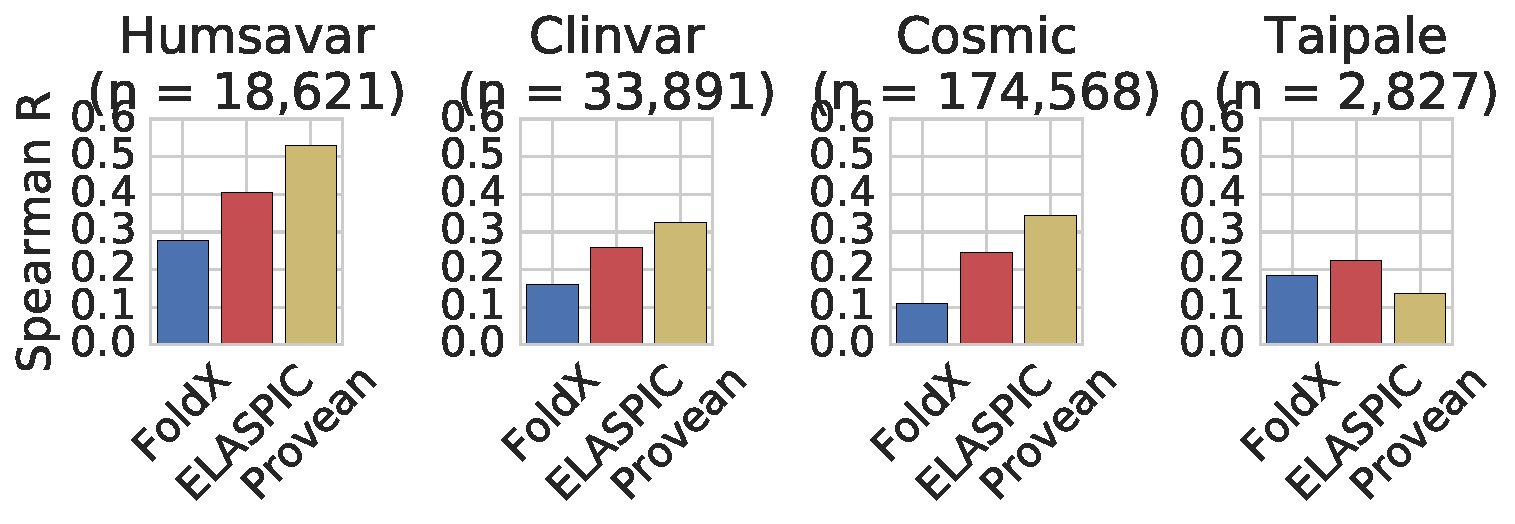
\includegraphics[width=0.8\textwidth]{static/elaspic_training_set/validation/validation_performance_core.pdf}
		\caption{
			Performance of the ELASPIC core predictor, FoldX and Provean on the validation datasets.
		}
		\label{fig:validation_performance_core}
		\vspace*{10mm}
	\end{subfigure}
	\begin{subfigure}[b]{1.0\textwidth}
		\centering
		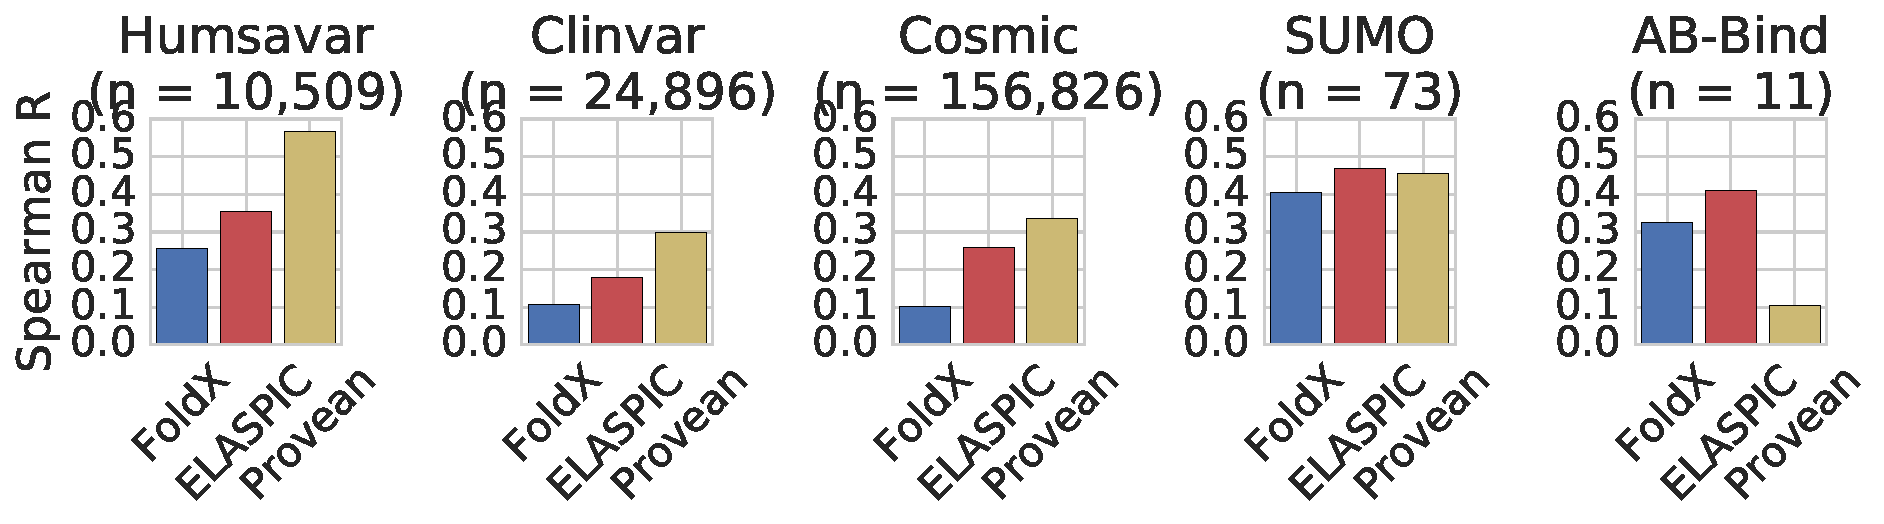
\includegraphics[width=1.0\textwidth]{static/elaspic_training_set/validation/test_performance_core.pdf}
		\caption{
			Performance of the ELASPIC core predictor, FoldX and Provean on the test datasets.
			There is no overlap in mutations (or proteins for Humsavar, ClinVar and COSMIC) between the test datasets,
			and the training and validation datasets (see Figure \ref{fig:training_set_overlap_core}).
		}
		\label{fig:test_performance_core}
		\vspace*{5mm}
	\end{subfigure}
	\caption[Core predictor validation.]{Performance of the ELASPIC core predictor on the training (a), validation (b) and test (c) datasets.}
	\label{fig:core_validation}
\end{figure}

\clearpage

\begin{figure}[tb]
	\centering
	\begin{subfigure}[b]{1.0\textwidth}
		\centering
		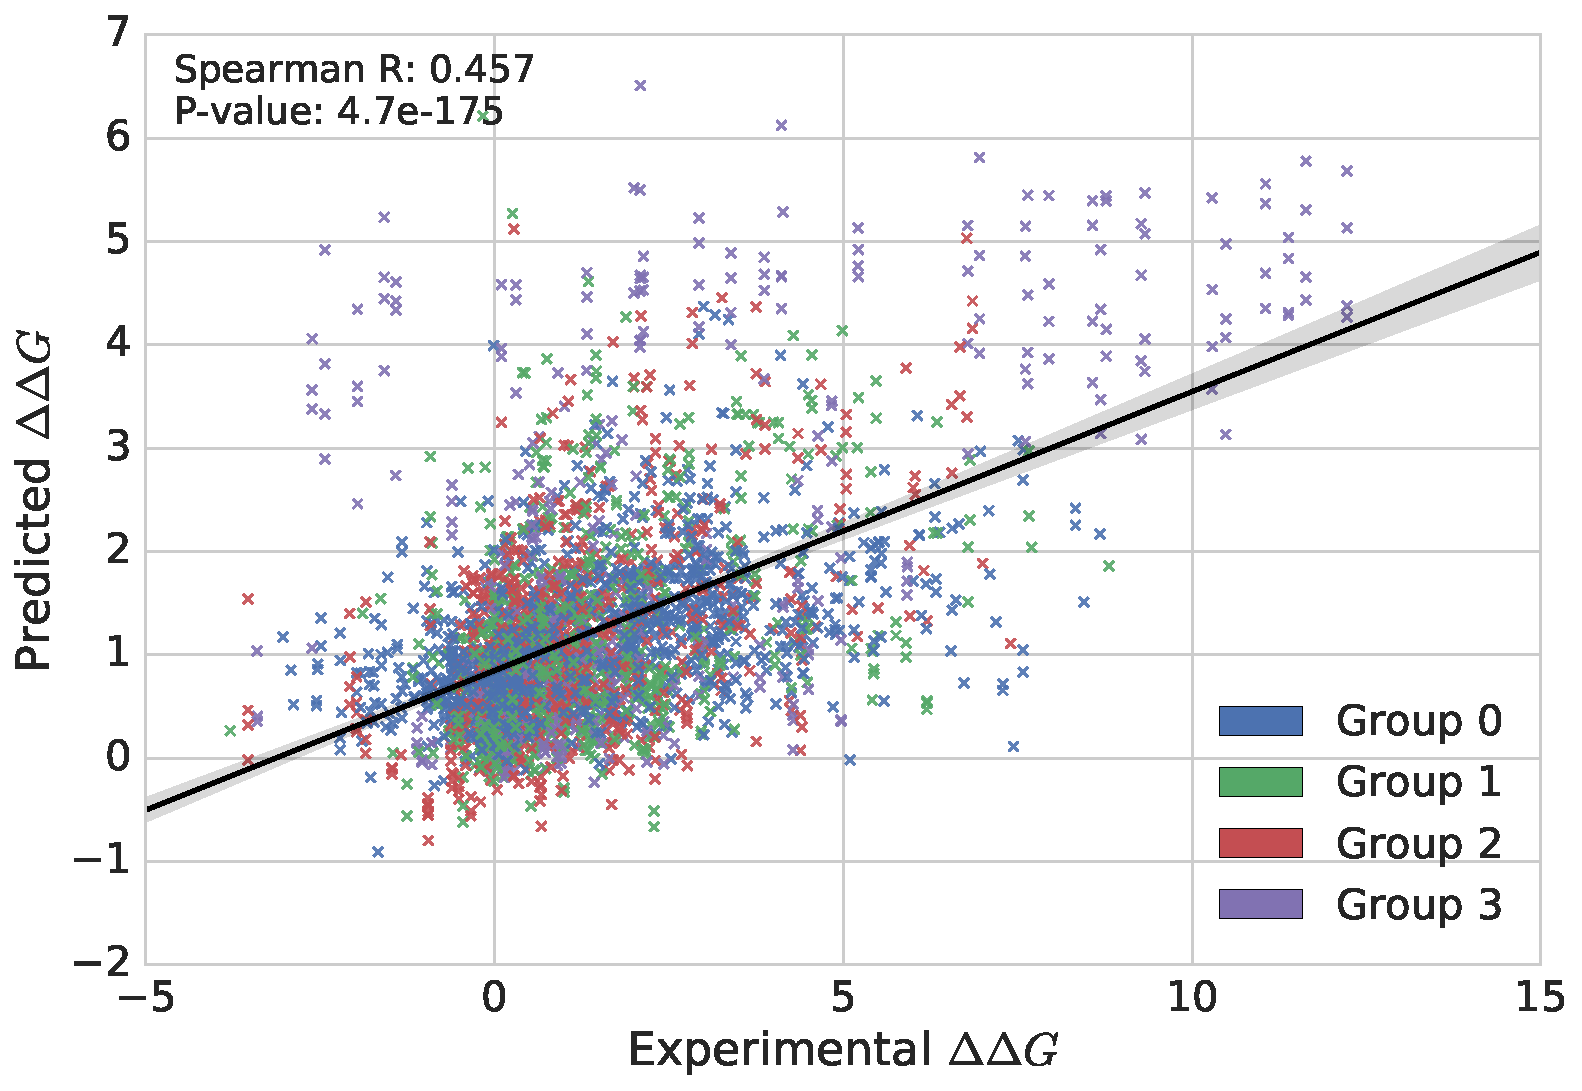
\includegraphics[width=0.6\linewidth]{static/elaspic_training_set/validation/crossvalidation_performance_interface.pdf}
		\caption{
			Performance of the ELASPIC interface predictor on the training dataset, evaluated using four-fold cross-validation.
			Colours indicate different cross-validation bins.
		}
		\label{fig:crossvalidation_performance_interface}
		\vspace*{10mm}
	\end{subfigure}
	\begin{subfigure}[b]{1.0\textwidth}
		\centering
		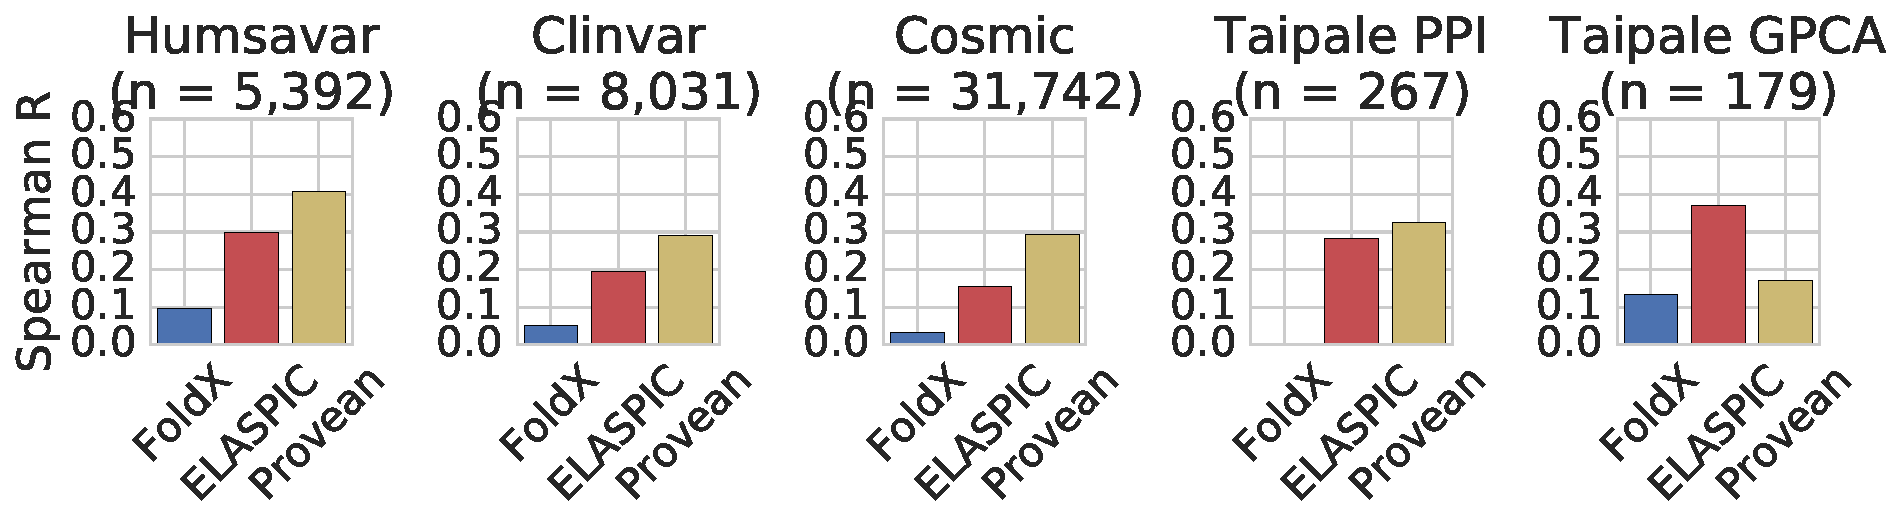
\includegraphics[width=0.9\textwidth]{static/elaspic_training_set/validation/validation_performance_interface.pdf}
		\caption{
			Performance of the ELASPIC interface predictor, FoldX and Provean on the validation datasets.
		}
		\label{fig:validation_performance_interface}
		\vspace*{10mm}
	\end{subfigure}
	\begin{subfigure}[b]{1.0\textwidth}
		\centering
		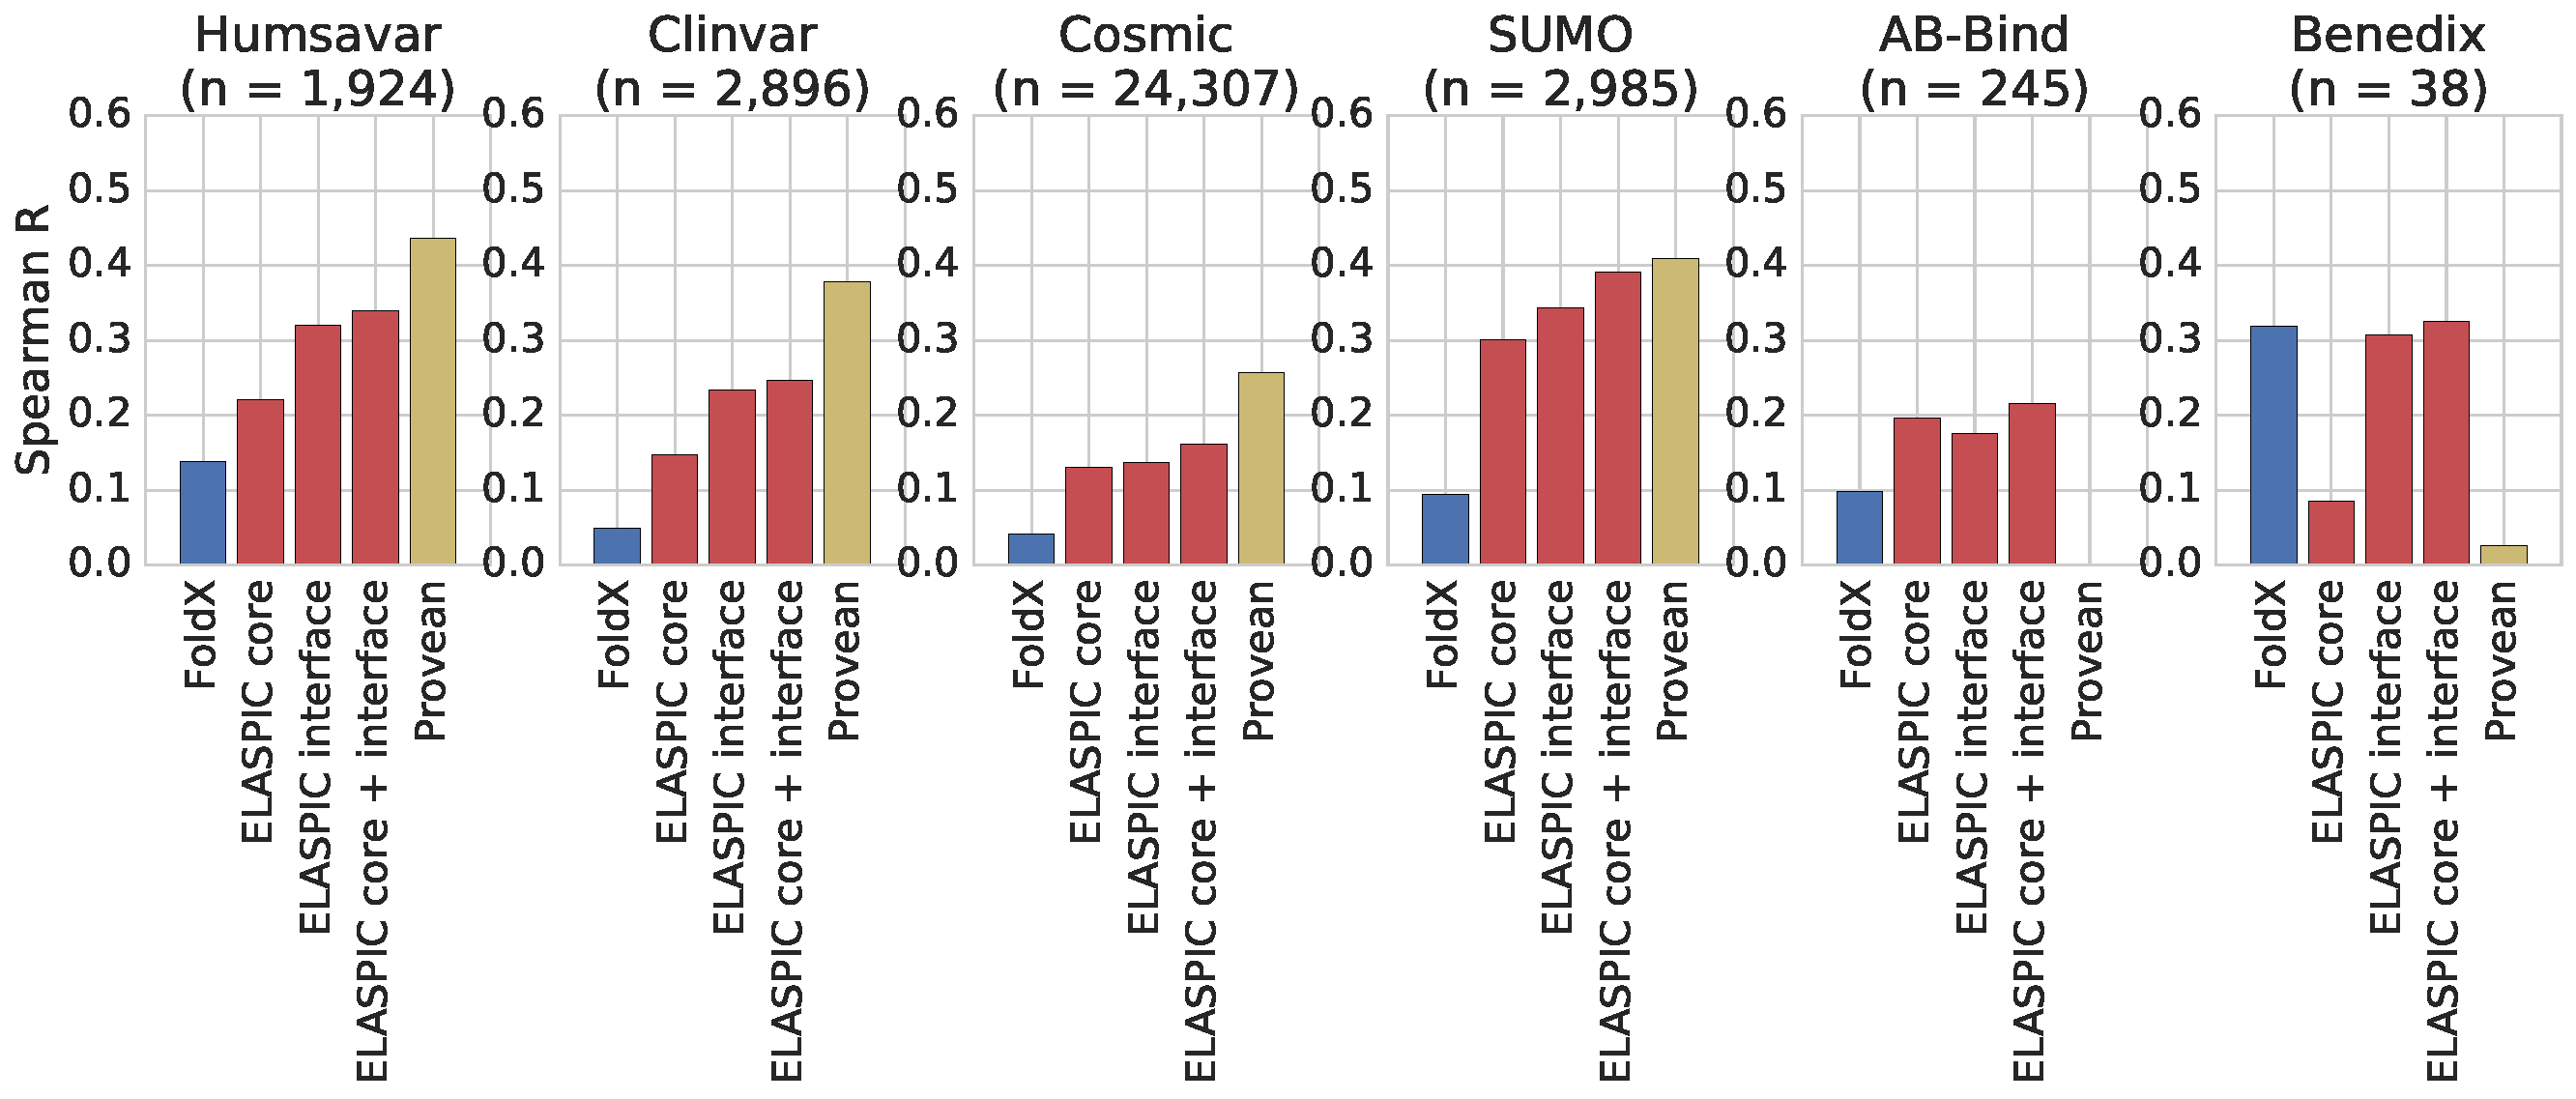
\includegraphics[width=1.0\textwidth]{static/elaspic_training_set/validation/test_performance_interface.pdf}
		\caption{
			Performance of ELASPIC, FoldX and Provean on the test datasets.
			Correlations are provided for core predictors, interface predictors, and the sum of core and interface predictors, for ELASPIC and FoldX.
			There is no overlap in mutations (or proteins for Humsavar, ClinVar and COSMIC) between the test datasets,
			and the training and validation datasets (see Figure \ref{fig:training_set_overlap_interface}).
		}
		\label{fig:test_performance_interface}
		\vspace*{5mm}
	\end{subfigure}
	\caption[Interface predictor validation.]{Performance of the ELASPIC interface predictor on the training (a), validation (b) and test (c) datasets.}
	\label{fig:interface_validation}
\end{figure}

